\documentclass[12pt
]{amsbook}

% \RequirePackage{geometry}
% \geometry{
%     headheight=4ex,
%     includehead,
%     includefoot
% }
% \raggedbottom
% \geometry{
%     paper=b5paper,
%     inner=30mm,         % Inner margin
%     outer=30mm,         % Outer margin
%     bindingoffset=10mm, % Binding offset
%     top=20mm,           % Top margin
%     bottom=28mm,        % Bottom margin
%     %showframe,         % show how the type block is set on the page
% }

\raggedbottom

\title{A universality criterion for integral quadratic forms}
\author{Roel Christian G. Yambao}
\date{November 2023}

\RequirePackage{amsmath}
\RequirePackage{amssymb}
\RequirePackage{amsfonts}
\RequirePackage{amsthm}


\RequirePackage[backend=biber]{biblatex}
\RequirePackage[pagestyles]{titlesec}
\RequirePackage{xcolor}
\RequirePackage{titletoc}

\RequirePackage{hyperref}
\hypersetup{
    colorlinks = true,
    linkcolor = green!50!black,
    anchorcolor = green!50!black,
    citecolor = green!50!black,
    filecolor = green!50!black,
    urlcolor = green!50!black
    }

\RequirePackage{graphicx}
\RequirePackage{subcaption}
\renewcommand{\figurename}{Fig.}
\renewcommand{\contentsname}{Contents.}
\renewcommand{\listfigurename}{List of figures.}
\DeclareCaptionFormat{custom}
{%
    {\footnotesize{\lsstylehelp{150}\scshape{{#1#2}}}\textit{#3}}
}
\captionsetup{format=custom}

\RequirePackage{enumitem}

\RequirePackage{tabularx}
\RequirePackage{mathrsfs}

% Only list chapters and sections in the ToC
\setcounter{tocdepth}{1}

% Section format in ToC
\titlecontents{section}
    [0pt]
    {}
    {\quad}
    {}
    {\titlerule*[1pc]{.}\contentspage}



\RequirePackage{fancyhdr}
\RequirePackage{extramarks}
\pagestyle{fancy}
\fancyhf{}
\renewcommand{\headrulewidth}{0pt}
\fancyhead[LE,RO]{\footnotesize\thepage}
\fancyhead[CE]{\scshape \MakeLowercase{\leftmark}}
\fancyhead[CO]{\scshape\MakeLowercase{\rightmark}}

\makeatletter
\renewcommand{\chaptermark}[1]{%
  \markboth{%
    \ifnum\c@secnumdepth>\m@ne
      \@chapapp\ {\small\thechapter}. \ %
    \fi
  #1%
  }{}%
}
\makeatother

\makeatletter
\renewcommand{\chaptermark}[1]{%
        \markboth{\thechapter.\ #1}{}}
% unnumbered chapters in the header
\renewcommand{\chaptermark}[1]{%
        \markboth{#1}{}}
        
\renewcommand{\sectionmark}[1]{\markright{\small #1}}
\renewcommand{\thepage}{\footnotesize\arabic{page}}
\makeatother



\RequirePackage[norule,symbol,perpage]{footmisc}
\RequirePackage{microtype}
\SetTracking{encoding=*, shape=sc}{60}
\widowpenalty10000
\clubpenalty10000
\usepackage{url}
\urlstyle{same}

% \RequirePackage[
%   oldstylenums, largesmallcaps
% ]{kpfonts}



% \usepackage[math-style=ISO]{unicode-math}
% \defaultfontfeatures{Mapping=tex-text}
% \DisableLigatures{encoding = *, shape = sc*}
% \setmainfont[Ligatures={Common,TeX},
% SmallCapsFeatures={
%   LetterSpace=7.5
% }]{Latin Modern}
% \setmathfont[Scale=0.97,Ligatures=TeX,
% math-style=TeX
% ]{Latin Modern Math}
% % \setmathfont[range=it/{Latin,latin}]{Linux Libertine O Italic}
% % % \setmathfont[range=up]{Junicode}
% % % \setmathfont[range=it/{Greek, greek}]{Linux Libertine O Italic}
% % \setmathfont[range=up/{Greek, greek}]{Linux Libertine O}
% % \setmathfont[range=it/{Greek, greek}]{Linux Libertine O Italic}
% \setmathfont[range=frak/{latin,Latin},
%                    Scale=MatchUppercase,
%                    StylisticSet=1,
%                    script-features={},
%                    sscript-features={}
%             ]{Unifraktur Maguntia}

% Theorem environments
\theoremstyle{plain}
\newtheorem*{theorem}{theorem}
\newtheorem*{lemma}{lemma}
\newtheorem*{corollary}{corollary}
% Numbered theorems
\newtheorem{theoremx}{theorem}[subsection]
\newtheorem{lemmax}{lemma}[subsection]
\newtheorem{corollaryx}{corollary}[subsection]
\newtheorem{corollaryb}{corollary}[subsection]



\theoremstyle{definition}
\newtheorem*{definition}{definition}

\renewenvironment{proof}{{\itshape Proof. }}{{\scshape q.e.d.}}

\RequirePackage{longtable}

\AtBeginDocument{
    \let\phi\varphi
    \let\epsilon\varepsilon
    \let\iff\Leftrightarrow
    \let\implies\Rightarrow
    \let\leq\leqslant
    \let\geq\geqslant
    \let\theta\vartheta
    \let\emptyset\varnothing
}

\addbibresource{../ref.bib}

\renewcommand{\thechapter}{\Roman{chapter}}
\renewcommand{\thesubsection}{\arabic{subsection}}

% \titleformat{\chapter}[display]
%     {\normalfont\centering}
%     {Chapter\,\thechapter.}{.5em}{\Large\scshape}
\makeatletter
\newcommand\lsstylehelp[1]{\edef\MT@letterspace@{#1}\lsstyle}
\makeatother

\titleformat{\chapter}[display]
{\normalsize\scshape\centering\lsstylehelp{500}}
{\centering\MakeLowercase{\chaptertitlename\:\thechapter.}\lsstylehelp{300}}
{0.5em}{\large\MakeUppercase}

\titleformat{\section}[block]
    {\normalfont\itshape\centering}
    {}
    {.5em} %
    {} 
    []

\titleformat{\subsection}[runin]
    {\bfseries}
    {\thesubsection.}{.5em}
    {}
    []
    
% Renew

\titlespacing*{\section}
{0pt}%
{6ex plus 1ex minus .2ex}
{4pt}

\titlespacing{\subsection}
    {\parindent}{1.5ex plus .1ex minus .2ex}{0pt}

\usepackage{chngcntr}
\counterwithout{equation}{chapter}
\counterwithout*{section}{chapter}
\counterwithout*{subsection}{section}
\counterwithout{theoremx}{chapter}
\counterwithout{corollaryx}{chapter}
\counterwithout{lemmax}{chapter}
\counterwithout{corollaryb}{chapter}
\counterwithout{figure}{chapter}
% do not reset theorem counter at each section
\renewcommand{\thetheoremx}{\scshape\roman{theoremx}}
\renewcommand{\thecorollaryx}{\scshape\alph{corollaryx}}
\renewcommand{\thelemmax}{\scshape\alph{lemmax}}

\renewcommand{\thecorollaryb}{\scshape\alph{corollaryb}} % additional corollary counter

\RequirePackage{etoolbox}
\renewcommand*{\bibfont}{\footnotesize}

\begin{document}

\thispagestyle{empty}
{\centering

    % DLSU Logo
    % 
\includegraphics[width=0.1\textwidth]{logo.png}

    % \vspace*{0.1in}

    {
        De La Salle University\\
        2401 Taft Avenue, Manila
    }

    \vspace*{2in}

    {\lsstylehelp{200}
        \Large
        A UNIVERSALITY CRITERION

        \vspace*{0.15in}
        
        FOR INTEGRAL QUADRATIC FORMS
    }

    \vspace*{0.2in}

    {\itshape
        \normalsize
        An exposition of Manjul Bhargava's proof\\
        of the Conway-Schneeberger Fifteen Theorem
    }

    \vspace*{0.2in}

    \vspace*{\fill}

    {
        \large
       Math 621 (Number Theory) --- Expository Paper
    }

    \vspace*{0.15in}


    {
        Roel Christian G. Yambao, November 2023
    }

    
}

\frontmatter
\cleardoublepage

\tableofcontents
\let\origaddvspace\addvspace
\renewcommand{\addvspace}[1]{}
\listoffigures
\renewcommand{\addvspace}[1]{\origaddvspace{#1}}

\cleardoublepage

\chapter*{Preface.}

{\scshape The aim} of this paper is to provide a self-contained exposition of the proof of the Conway-Schneeberger Fifteen Theorem provided by Manjul Bhargava in \cite{bhargava2000conway}. The theorem states that for a positive-definite integer-valued quadratic form to represent all positive integers, it is necessary and sufficient that it represent all positive integers up to \(15\). The original proof by Conway was never published, although in 1995, William Schneeberger has provided a sketch of the proof in his Ph.D. thesis. \cite{schneeberger1997arithmetic} The proof we examine here was provided by Bhargava in 2000, relying heavily on the theory of genera and of lattices; Bhargava was later to generalize this in what would later be known as the \(290\) theorem. \cite{bhargava2005universal} For this and his other contributions to number theory, in particular to the geometry of numbers, Bhargava was awarded the Fields Medal in 2014. \cite{bhargava2014fields}

While the author has endeavoured to make this exposition as self-contained as possible, some elementary results have been omitted and throughout the paper, the reader will be assumed to have a basic understanding of number theory, linear algebra, and abstract algebra, on the level of the introductory graduate courses on those subjects in De La Salle University. 

Chapter \ref{chap:quadratic-forms} provides an introduction of the theory of quadratic forms over a field \(\field\) of characteristic not equal to \(2\) and the equivalent notions of Gram matrices and symmetric bilinear forms, following the treatment in \cite{lam1973quadratic}. The main results in the chapter include the equivalence of quadratic forms to a diagonal form as well as some results specific to the number theoretic treatment of rational and integral quadratic forms from \cite{cassels2008rational} and \cite{jones1950arithmetic}. Chapter \ref{chap:local-global-principle} is essentially an exposition of Chapters 2--4 of Serre's \emph{Course in Arithmetic} \cite{serre2012course}. In it, we construct the field \(\Rationals_p\) of \(p\)-adic numbers, develop the theory of quadratic forms in \(\Rationals_p\) and \(\Rationals\), and finally prove the Hasse-Minkowski theorem. We then explore some consequences of this theorem and its applications to number theory. In Chapter \ref{chap:integral-quadratic-forms} we introduce the language of lattices to study quadratic forms over the the rings \(\Integers\) and \(\Integers_p\) in order to investigate how, if at all possible, to extend the results of Chapter \ref{chap:local-global-principle} to analogues for principal ideal domains, in particular \(\Integers\). The exposition in this chapter follows closely the treatment in \cite{cassels2008rational,gerstein2008basic,jones1950arithmetic}. Chapter \ref{chap:conway-schneeberger} uses the results of the previous chapters to prove the Conway-Schneeberger Fifteen Theorem using the method of escalating lattices. We follow the original exposition in \cite{bhargava2000conway}, as well as \cite{moon2008universal}. We conclude by quickly reviewing the \(290\) theorem of Bhargava and Hanke \cite{bhargava2005universal}, which generalizes the Fifteen Theorem for integral quadratic forms (in the sense of \S\,\ref{sec:integral-forms-def}).


\begin{figure}
    \centering
    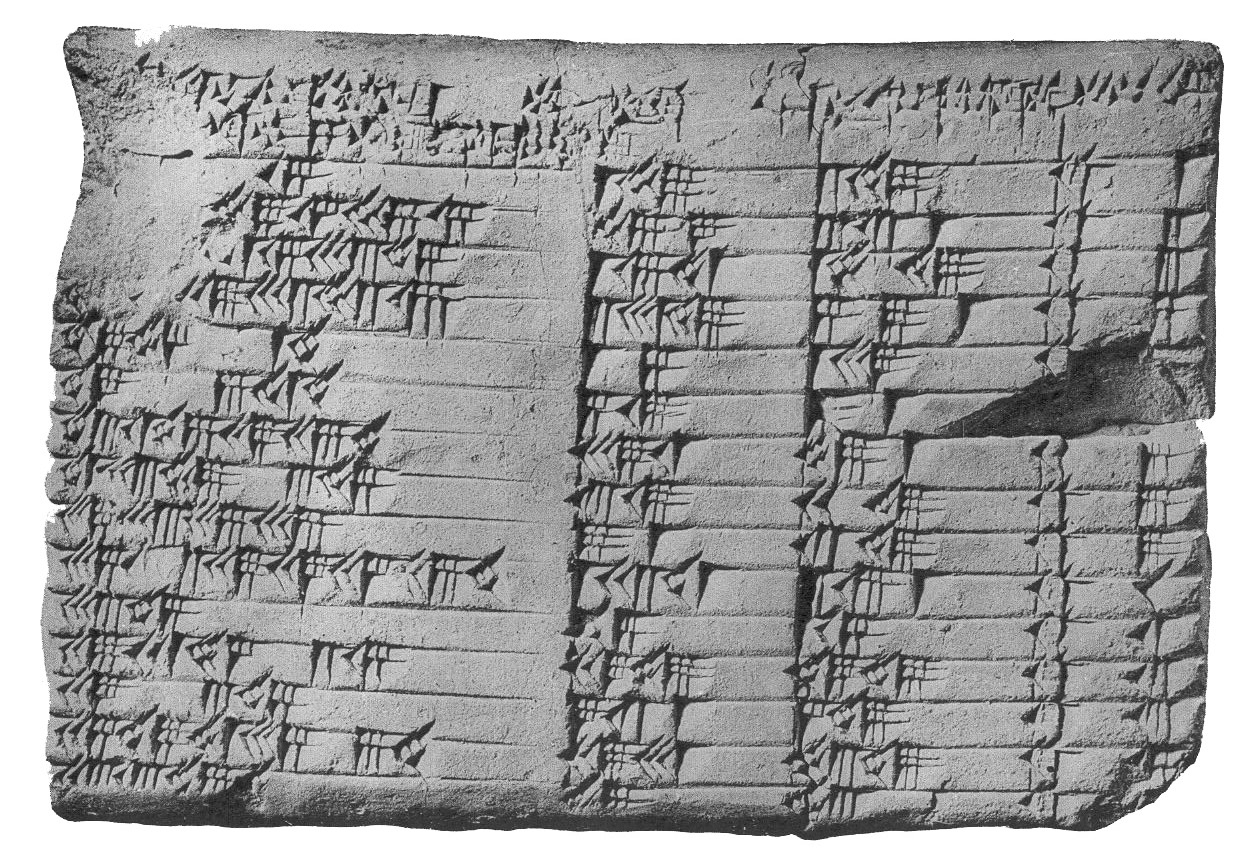
\includegraphics[width=\textwidth]{assets/Plimpton_322.jpg}
    \caption[The Plimpton 322 tablet.]{The Plimpton 322 tablet. Image from Wikimedia Commons.}
    \label{fig:plimpton-322}
\end{figure}

\begin{figure}
    \centering
    \includegraphics[width=0.8\textwidth]{assets/euclid.png}
    \caption[A geometric construction of Pythagorean triples.]{A geometric construction of Pythagorean triples from Euclid's \emph{Elements}. Image from the Greek text prepared by Heiberg. \cite{heiberg1885euclid}}
    \label{fig:pythagorean-triples}
\end{figure}

\section*{A historical note.}


A quadratic form is a homogeneous polynomial of degree two (form, in this case, being a dated term for a homogeneous polynomial). The theory of quadratic forms has a long and rich history, with some of the earliest results dating back to antiquity. For example, integer solutions to the equation
\[
    x^2 + y^2 = z^2 
\]
have been known to the ancient Babylonians,referred to as Pythagorean triples, although the results likely predate the Pythagoreans. A table of fifteen triples have been preserved in a tablet that has come to be labelled as Plimpton 322 (after its provenance) and has been dated to between the 19th and 16th centuries {\lsstylehelp{100}\sc b.c.e.} \cite{robson2002words} Euclid (fl. 300 {\lsstylehelp{100}\sc b.c.e.}), in Book X, Prop.\,29, of his \emph{Elements}, has demonstrated a way of constructing Pythagorean triples geometrically. \cite{euclid1956elements} Following Euclid, the next substantial treatment of quadratic forms (and of classical number theory, in general) was given by Diophantus of Alexandria in his \emph{Arithmetica}, which has served as the prototypical number theory text for much of antiquity and the Middle Ages. \cite{katz2009history} Thus for any pair of integers \(m\) and \(n\) with \(m > n\), the triple
\(
    (2mn, m^2 - n^2, m^2 + n^2)
\)
is a Pythagorean triple. These results has been attested to have developed separately in the Indian and Chinese mathematical traditions as well. \cite{weil1984number}

The work of Diophantus on the theory of numbers continued to be expanded upon both by Islamic mathematicians during the Middle Ages, including in treatises by al-Khwarizmi (fl. 800 {\lsstylehelp{100}\sc c.e.}) and European mathematicians like Vi\`ete, Bachet, and Pacioli during the Renaissance. In the 18th century, Pierre de Fermat and Leonhard Euler have shown that all prime numbers of the form \(4n + 1\) can be represented by a sum of squares.\,\cite{hahn2008quadratic} Later on Fermat and Joseph-Louis Lagrange have expanded this to sums of the form \(x^2 + Ny^2\) for some integer \(N\). Perhaps the most famous result of this period is Lagrange's assertion that every whole number can be expressed as the sum of four squares. Fermat, during this time, has introduced one of the longest-standing open problems in number theory, his ``last theorem'' about how there are no integer solutions to the equation \(x^n + y^n = z^n\) for \(n > 2\). While this problem is not directly related to quadratic forms, it has significantly influenced the development of the theory of numbers in the centuries since, culminating in a solution by Andrew Wiles in 1995. \cite{wiles1995modular}

At the turn of the century, Carl Friedrich Gauss published what was to become the most influential work on number theory, \emph{Disquisitiones Arithmetic\ae}. It is difficult to overstate the effect that Gauss’s \emph{Disquisitiones} has had on the development of the theory of numbers. This work is to cast a long shadow on the work of mathematicians in the the time since its original publication, not least because of the sheer scope of its contents. Two centuries after \emph{Disquisitiones} first appeared, the mathematician John Conway was to remark, for example,
\begin{quote}
    [W]hen Neil Sloane and I wanted to summarize the classification theory of binary forms for one of our books, we found that the only Number Theory textbook in the Cambridge Mathematical Library that handled every case was still the \emph{Disquisitiones}! \cite{conway1999universal} 
\end{quote}
In \emph{Disquisitiones}, Gauss has introduced, among other things, important results in congruence,\,---\,a notion which remains a central concept in modern number theory; much of the number theoretic notation still used to this day can be traced back to this book by Gauss, in particular writing
\[
    a \equiv b \quad (\text{mod. } m)
\]
to indicate that \(a\) and \(b\) are ``congruent'' under the  ``modulus'' \(m\). (The dot after the original abbreviation was soon to disappear.) More than half of the six-hundred-odd pages of \emph{Disquisitiones} is devoted to the theory of quadratic forms and quadratic reciprocity, which Gauss has exhaustively studied. 

Throughout the nineteenth century, work on quadratic forms continued, building on the foundations laid by Gauss. The reduction and classification theories in the \emph{Disquisitiones} was completed by James Joseph Sylvester (in his famous ``law of inertia'') over the real numbers. The French mathematician Charles Hermite has provided useful bounds for reducing quadratic forms over \(\Integers\) using the concept of the minimum of a positive-definite quadratic form. \cite{gerstein2008basic} (We shall review some of these results in Chapter \ref{chap:quadratic-forms}.) Towards the end of the nineteenth century, Hermann Minkowski introduced the ``local-global'' principle for the classification of quadratic forms. The introduction by Kurt Hensel in 1897 of \(p\)-adic numbers, and the work on valuation theory by his student Helmut Hasse, has allowed for the extension of the local-global principle to a more general number-theoretic setting. \cite{gerstein2008basic,hensel1913zahlentheorie,hasse1922uber} We shall develop the results from Minkowski, Hensel, and Hasse as they apply to quadratic forms in Chapter \,\ref{chap:local-global-principle}.
\chapter*{Notation}

{\itshape\quad The page numbers refer to the page where the notation is first defined or used (excluding the preface).}

\bigskip

\begin{longtable}{p{0.25\linewidth} p{0.01\linewidth} p{0.65\linewidth}}
    \(\field\) && a field, p.\,\pageref{sec:quadratic-forms}\\
    \(\Rationals\) && the field of rational numbers, p.\,\pageref{sec:quadratic-forms}\\
    \(q, r, s, q', r', s',\) etc. && quadratic forms, p.\,\pageref{sec:quadratic-forms}\\
    \(\field[x_1, \dots, x_n]\) && the ring of polynomials in \(n\) variables over \(\field\), p.\,\pageref{sec:quadratic-forms}\\
    \(A = (a_{ij})\) && the matrix \(A\) with entries \(a_{ij}\), p.\,\pageref{sec:quadratic-forms-matrix-representation}\\
    \(x^{\transp}, M^{\transp}\) && the transpose of the vector \(x\) and the matrix \(M\), respectively, p.\,\pageref{sec:quadratic-forms-matrix-representation}\\
    \(\field^n\) && the direct sum of \(n\) copies of \(\field\), often interpreted as a vector space, p.\,\pageref{sec:quadratic-forms-matrix-representation}\\
    \(\discr q\) && the discriminant of the quadratic form \(q\), p.\,\pageref{sec:quadratic-forms-matrix-representation}\\
    \(A \to B\) && a map from \(A\) to \(B\), p.\,\pageref{sec:quadratic-maps}\\
    \(A \times B\) && the Cartesian product of \(A\) and \(B\), p.\,\pageref{sec:quadratic-maps}\\
    \(V\) && a (finite-dimensional) vector space, p.\,\pageref{sec:quadratic-maps}\\
    \((V, B)\) && a quadratic space, p.\,\pageref{sec:quadratic-maps}\\
    \(B(x, y)\) && the image under the bilinear form \(B\) of the pair \((x, y)\), p.\,\pageref{sec:quadratic-forms-basis}\\
    \(\Basis = \{b_1, \dots, b_n\}\) && a basis of a vector space, p.\,\pageref{sec:quadratic-forms-basis}\\
    \(\genlin{n}{\field}\) && the general linear group of degree \(n\) over \(\field\), i.e., the group of invertible \(n \times n\) matrices over \(\field\), p.\,\pageref{sec:quadratic-space-change-of-basis}\\
    \(\det M\) && the determinant of the matrix \(M\), p.\,\pageref{sec:quadratic-space-change-of-basis}\\
    \(\fieldU\) && the multiplicative group of units of \(\field\), p.\,\pageref{sec:square-classes}\\
    \(\SquareClass\) && the set of square classes of \(\field\), p.\,\pageref{sec:square-classes}\\
    \(D(q)\) && the set of all elements of \(\field\) that are represented by the quadratic form \(q\), p.\,\pageref{sec:representation}\\ 
    \(V^*\) && the dual space of \(V\), p.\,\pageref{sec:nondegenerate}\\
    %\(f\,_{|A}\) && the restriction of the map \(f\) to the set \(A\), p.\,\pageref{sec:orthogonality}\\
    \(W^{\perp}\) && the orthogonal complement of the subspace \(W\) (of a vector space \(V\)), p.\,\pageref{sec:orthogonality}\\
    \(\Radical V\) && the radical of the vector space \(V\), p.\,\pageref{sec:orthogonality}\\
    \(\dim V\) && the dimension of the vector space \(V\), p.\,\pageref{sec:orthogonality}\\
    \(V \oplus W\) && the direct sum of the vector spaces \(V\) and \(W\), p.\,\pageref{sec:orthogonal-sum}\\
    && or, the block sum of the matrices \(V\) and \(W\), p.\,\pageref{eq:orthogonal-sum-as-block-sum}\\
    \(V \perp W\) && the orthogonal sum of the quadratic spaces \(V\) and \(W\), p.\,\pageref{sec:orthogonal-sum}\\
    \(\quadform{\lambda}\) && the isometry class of \(\lambda\), p.\,\pageref{sec:lambda-class}\\
    \(\quadform{\lambda_1, \dots, \lambda_n}\) && the quadratic form equivalent to the form \(\lambda_1 x_1^2 + \dots + \lambda_n x_n^2\), i.e., the orthogonal sum \(\quadform{\lambda_1} \perp \dots \perp \quadform{\lambda_n}\), p.\,\pageref{sec:lambda-class}\\
    \(\min q\) && the minimum of the quadratic form \(q\), p.\,\pageref{sec:minimum}\\
    \(|a|\) && the absolute value of the number \(a\), p.\,\pageref{sec:minimum}\\
    \(p\) && a prime number, p.\,\pageref{chap:local-global-principle}\\
    \(\Rationals_p\) && the field of \(p\)-adic numbers, p.\,\pageref{chap:local-global-principle}\\
    \(\Integers_p\) && the ring of \(p\)-adic integers, p.\,\pageref{chap:local-global-principle}\\
    \(\Integers\) && the ring of integers, p.\,\pageref{chap:local-global-principle}\\
    \(\Integers/m\Integers\) && the ring of integers modulo \(m\), p.\,\pageref{chap:local-global-principle}\\
    \(\varprojlim A_i\) && the inverse limit of the projective system \(A_i\), p.\,\pageref{chap:local-global-principle}\\
    \(a \mid b\) && \(a\) divides \(b\), p.\,\pageref{thm:criterion-units-of-zp}\\
    \(\Units\) && the units of the ring \(\Integers_p\), p.\,\pageref{thm:criterion-units-of-zp}\\
    \(\Integers_{\geq 0}\) && the set of nonnegative integers, p.\,\pageref{thm:criterion-units-of-zp}\\
    \(\nu_p\) && the \(p\)-adic valuation, p.\,\pageref{thm:criterion-units-of-zp}\\
    \(|x|_p\) && the \(p\)-adic absolute value of \(x\), p.\,\pageref{thm:criterion-units-of-zp}\\
    \(\Integers_p^m\) && the set of \(m\)-tuples of \(p\)-adic integers, p.\,\pageref{thm:criterion-units-of-zp}\\
    \((a, b)\) && the Hilbert symbol of \(a\) and \(b\), p.\,\pageref{sec:hilbert-symbol}\\
    \(\FiniteField_q\) && the finite field of order \(q\), p.\,\pageref{sec:results-from-witt}\\
    \(\epsilon\) && the Hasse-Minkowski invariant of a quadratic form, p.\,\pageref{sec:hasse-invariant}\\
    \(\Places\) && the set of all places of \(\Rationals\) or \(\Integers\), i.e., the union of the set of all prime numbers and the symbol \(\infty\), p.\,\pageref{sec:hasse-minkowski}\\
    \(\Lattice\) && an \(R\)-lattice in a vector space \(V\), p.\,\pageref{sec:lattice}\\
    % \(\Rationals_p^{\times}\) && the of units of the field \(\Rationals_p\), p.\,\pageref{thm:criterion-units-of-zp}\\
\end{longtable}

\cleardoublepage

\mainmatter

%\chapter{Quadratic forms.}
\label{chap:quadratic-forms}

\section{Fundamental notions.}

{\scshape We begin} by presenting four definitions of a quadratic form and show
that they are equivalent. This allows us to freely switch between these
definitions as needed. The classical results on quadratic forms presented in
this chapter have been adapted from
\cite{clarkquadratic,lam1973quadratic,ormsbynotes,szymiczek2017bilinear}.

\subsection{}\label{sec:quadratic-forms}~Let \(\field\) be a field with
characteristic not equal to \(2\) (we maintain this assumption throughout this
paper, unless otherwise stated). A \emph{quadratic form} over \(\field\) is an
element \(q \in \field[x_1, \dots, x_n]\) of the polynomial ring in \(n\)
variables with coefficients in \(\field\) such that \(q\) can be written as
\[
  q(x_1, \dots, x_n) = \sum_{i, j} a_{ij}x_ix_j,
\]
for some \(a_{ij} \in \field\). That is, \(q\) is a homogeneous (i.e., all terms
have the same degree) polynomial of degree \(2\). For example, the polynomial
\(x^2 + 2xy + 3y^2\) is a binary quadratic form over \(\field = \Rationals\),
while \(x^2 + 2x + 3y\) is not. We call \(n\) the \emph{rank} of the quadratic
form \(q\). We shall often abbreviate the column vector \((x_1, \dots, x_n)\) as
\(x\) (and \(q(x_1, \dots, x_n)\) as \(q(x)\) or simply \(q\)). We shall also
follow convention and call quadratic form of rank \(n\) binary, ternary, or
quaternary if \(n = 2, 3, 4\), respectively.

Observe that our definition of a quadratic form allows for some redundancies.
That is, for example, the forms \(3x^2 + 4xy - yx + 2y^2\) and \(3x^2 + xy + 2yx
+ 2y^2\) are presentations of the same quadratic form. It is therefore customary
to ``symmetrize'' the form \cite{lam1973quadratic} by replacing the coefficients
\(a_{ij}\) with \(a'_{ij} = \frac{1}{2}(a_{ij} + a_{ji})\) (we are able to do so
as \(\charx \field \neq 2\) by assumption) so that given a quadratic form \(q\)
over \(\field\), we have
\[
  q = \sum_{i, j} a_{ij} x_i x_j = \sum_{i, j} a'_{ij} x_i x_j
\]
where \(a'_{ij} = a'_{ji}\) for all \(i, j\). Thus the forms \(3x^2 + 4xy - yx +
2y^2\) and \(3x^2 + xy + 2yx + 2y^2\) can be symmetrized to \[3x^2
+\frac{3}{2}xy + \frac{3}{2}yx + 2y^2.\] (And, since \(\field\) is a field, this
ultimately simplifies to \(3x^2 + 3xy + 2y^2\).)

This symmetrization allows us to associate a symmetric matrix \(M = (m_{ij})\)
to a quadratic form \(q\) over \(\field\) by letting \(m_{ij} = a'_{ij}\). The
matrix \(M\) is unique because it is uniquely determined by the coefficients of
\(q\) and is called the \emph{symmetric matrix associated with \(q\)}.
Conversely, from any nonzero \(n \times n\) matrix \(M\) we can define a
quadratic form \(q\) by
\[
  q(x) = x^{\transp}Mx
\]
where \(x\) is a column vector in \(\field^n\). The reader may verify that this
is indeed a quadratic form. We shall write \(\discr q\) to denote the
determinant of the symmetric matrix associated with \(q\) and call it the
discriminant of \(q\).\label{sec:quadratic-forms-matrix-representation}

\subsection{Another perspective.}~Evaluating the polynomial \(q\) at a vector
\(x \in \field^n\) can be seen as a map from \(\field^n\) to \(\field\). Thus
any quadratic form \(q\) over \(\field\) naturally induces a map \(\field^n \to
\field\), which with some abuse of notation we shall also denote by \(q\). This
map is called a \emph{quadratic map} and is ``quadratic'' in the sense
that\label{sec:quadratic-maps}
\[q(\lambda x) = \lambda^2q(x)\] for all \(\lambda \in \field\) and \(x \in
\field^n\). Indeed, we have \(q(\lambda x) = (\lambda x)^{\transp}M(\lambda x)
= \lambda^2 x^{\transp}Mx = \lambda^2 q(x).\) In addition, the map \(q\) has the
property that if we define a map \(B : \field^n \times \field^n \to \field\) by
\[
  B(x, y) = \frac{1}{2}\left(q(x+y) - q(x) - q(y)\right),
\]
then \(B\) is a \emph{symmetric bilinear form} over \(\field\). That is, \(B\)
is a bilinear map (i.e., linear in each argument) that satisfies
\[
  B(x, y) = B(y, x)
\]
for all \(x, y \in \field^n\). We call \(B\) the \emph{polarization} of (the
map) \(q\). That \(B\) is bilinear can be proved as follows:
\begin{align*}
  B(x,y) &= \frac{1}{2}\left(q(x+y) - q(x) - q(y)\right)\\
  &= \frac{1}{2}\left( (x+y)^{\transp}M(x+y) - x^{\transp}Mx - y^{\transp}My \right)\\
  &= x^{\transp}My.
\end{align*}

Conversely, given a symmetric bilinear form \(B\) over \(\field\), we can define
a quadratic form \(q\) by
\[B(x, x) = \frac{1}{2}\left(q(x+x) - q(x) - q(x)\right) =\frac{1}{2}\left(q(2x)
- 2q(x)\right) = q(x).\] Thus each of \(q\) and \(B\) uniquely determines the
other.

Our definitions have thus far been restricted to quadratic maps defined on
\(\field^n\) (and consequently symmetric bilinear forms on \(\field^n\)). If,
however, we define for any \(n\)-dimensional \(\field\)-vector space \(V\) the
symmetric bilinear form \(B: V \times V \to \field\) and associate it with the
quadratic map \(q:= q_B: V \to \field\) defined by \(q(x) = B(x,x)\), then we
have, for all \(x, y \in V\) and \(\lambda \in \field\),
\[
    q(\lambda x) = B(\lambda x, \lambda x) = \lambda^2 B(x, x) = \lambda^2 q(x),
\]
and
\begin{align*}
    q(x + y ) - q(x) - q(y) &= B(x+y, x+y) - B(x, x) - B(y, y)\\
    &=B(x,y) + B(y,x) = 2B(x,y).
\end{align*}
And thus we see that \(q\) is indeed a quadratic map and that each of \(q\) and
\(B\) uniquely determines the other. We shall call the pair \((V, B)\) a
\emph{quadratic space}.\footnote{The notation \((V, q)\) also appears in the
literature; cf., e.g., \cite[p.~4]{lam1973quadratic}.} Throughout this book, all
vector spaces will be understood to be finite.

Working with quadratic spaces allow us to deal with quadratic forms without
regard to a specific basis. Consider the quadratic space \((V, B)\) and let
\(\Basis = \{b_1, \dots, b_n\}\) be a basis of \(V\). This gives rise to the
quadratic form
\[
  q(x_1, \dots, x_n) = \sum_{i, j} B(b_i, b_j) x_i x_j,  
\]
and if we use the fact that \(V\) is isomorphic to \(\field^n\), then we can
identify \(q\) with the quadratic form \(q(x) = x^{\transp}Mx\) where \(M\) is
the matrix whose \(ij\)-th entry is \(B(b_i, b_j)\). Thus the map \(q_B : V \to
\field\) is precisely the quadratic map \(\field^n \to \field\) induced by
\(q\). We call \(M\) the \emph{Gram matrix} of \((V, B)\) with respect to the
basis \(\Basis\).\label{sec:quadratic-forms-basis}

If we let \((V, B)\) be a quadratic space and \(M\) and \(q\) be the Gram matrix
and quadratic map associated with \((V, B)\), in that order, with respect to the
basis \(\Basis =\{b_1, \dots, b_n\}\), then if we let \(\Basis' = \{b'_1, \dots,
b'_n\}\) be another basis of \(V\) and let \(M'\) and \(q'\) be the Gram matrix
and quadratic map associated with \((V, B)\), in that order, with respect to
\(\Basis'\), then we can express the basis vectors \(b'_i\) in terms of the
basis vectors \(b_i\), \emph{viz.,}\label{sec:quadratic-space-change-of-basis}
\begin{align*}
    b'_1 &= p_{11}b_1 + \cdots + p_{n1}b_n\\
    &\vdots\\
    b'_n &= p_{1n}b_1 + \cdots + p_{nn}b_n,
\end{align*}
so that the matrix \(P = (p_{ij})\) is the change of basis matrix from
\(\Basis\) to \(\Basis'\). Since \(\Basis\) and \(\Basis'\) are bases of the
same vector space, we know that \(P \in \genlin{n}{\field}\). We then have
\begin{align*}
  M' &= B(b'_i, b'_j) = B\left(\sum_{s} p_{si}b_s, \sum_t p_{tj}b_t\right)\\
  &= \sum_t \sum_s p_{si}B(b_s, b_t)p_{tj}.
\end{align*}
The term \(B(b_s, b_t)\) is the \(st\)-th entry of \(M\), \(m_{st}\), so that
\(c_{it} := \sum_s p^{\transp}_{si}m_{st}\) is the \(it\)-th entry of
\(P^{\transp}M\). Finally, \(\sum_t c_{it}p_{tj}\) is exactly the \(ij\)-th
entry of the matrix product \(P^{\transp}MP\). Thus the quadratic space \((V,
B)\) determines uniquely the equivalence class of the quadratic form \(q\).

\subsection{An illustration.}~It will be instructive to see how these four
definitions of a quadratic form are related. Consider the quadratic form \[q(x,
y) = x^2 + 4xy + 3y^2\] over \(\field = \Rationals\). We can symmetrize this to
\[q(x, y) = x^2 + 2xy + 2yx + 3y^2,\] which we can then associate to the
symmetric matrix \(M = \begin{pmatrix} 1 & 2 \\ 2 & 3 \end{pmatrix}\) so that
\[
  q(x, y) = \begin{pmatrix}
    x & y
  \end{pmatrix} \begin{pmatrix}
    1 & 2 \\
    2 & 3
  \end{pmatrix} \begin{pmatrix}
    x \\ y
  \end{pmatrix}= x^2 + 4xy + 3y^2,
\]
as expected. If \(\{e_1, e_2\}\) is the standard basis of \(\Rationals^2\), then
the associated quadratic map is given by \(xe_1 + ye_2 \mapsto x^2 + 4xy +
3y^2\). The polarization of this map is given by
\begin{align*}
  B((x,y), (x', y')) &= \frac{1}{2}\left(q((x,y) + (x', y')) - q((x,y)) - q((x', y'))\right)\\
  &= \frac{1}{2}\left(q(x+x', y+y') - q(x, y) - q(x', y')\right)\\
  &= xx' + 2xy' + 2x'y + 3yy',
\end{align*}
which when evaluated at a pair of standard basis vectors gives us the Gram
matrix \(B = \begin{pmatrix} 1 & 2 \\ 2 & 3 \end{pmatrix}\), as before. Finally,
depolarizing \(B\) gives us
\[
  B((x, y), (x, y)) = x^2 + 2xy + 2xy + 3y^2 = x^2 + 4xy + 3y^2.
\]

\section{Equivalence of forms.}

\subsection{Equivalence of forms.}\label{sec:mat-equiv}~Let \(\mathfrak{M}\) be
the set of all \(n \times n\) matrices over an arbitrary field \(\field\) of
characteristic not equal to \(2\). Given a matrix \(M \in \mathfrak{M}\) and a
quadratic form \(q\) of rank \(n\) over the same field \(\field\), we can define
a new quadratic form \(q'\) by
\begin{equation}\label{eq:mat-action}
  q'(x) := q(Mx) = q\left(\sum_{1 \leq i \leq n} m_{1i}x_i, \dots, \sum_{1 \leq i \leq n} m_{ni}x_i\right).
\end{equation}
so that the change from \(q\) to \(q'\) is merely that of linearly changing the
variables from \(x\) to \(Mx\). If we let \(N\) and \(N'\) be the matrices
associated with \(q\) and \(q'\), respectively, then we have
\[
  q'(x) = x^{\transp}N'x = (Mx)^{\transp}N(Mx) = x^{\transp} M^{\transp}NMx,
\]
and therefore
\begin{equation}\label{eq:mat-equiv}
  N' = M^{\transp}NM.
\end{equation}
Matrices \(N\) and \(N'\) satisfying Equation (\ref{eq:mat-equiv}) are said to
be \emph{congruent}.

Observe that if \(I\) is the identity matrix in \(\mathfrak{M}\) then \(q(Ix) =
q(x)\). Moreover, if \(M_1\) and \(M_2\) are matrices in \(\mathfrak{M}\) then
\(q((M_1M_2)x) = q(M_1(M_2x))\). If we restrict our consideration to only those
matrices in \(\frak{M}\) which are invertible (i.e., the general linear group
\(\genlin{n}{\field}\)), then we can observe that (\ref{eq:mat-action}) defines
a group action of \(\genlin{n}{\field}\) on the set of quadratic forms over
\(\field\).

This group action allows us to define an equivalence relation
\cite[p.~89]{hungerford2012algebra} on the set of quadratic forms over
\(\field\) as follows: we say that two quadratic forms \(q\) and \(r\) are
\emph{equivalent} (or more precisely, \emph{\(\genlin{n}{\field}\)-equivalent})
if there exists a matrix \(P \in \genlin{n}{\field}\) such that \(q(x) =
r(Px)\). In such a case, we write \(q \sim r\).

We claim, for example, that the forms \(q(x, y) = xy\) and \(r(x, y) = x^2 -
y^2\) are equivalent. Indeed, we have
\[
  q(x+y, x-y) = (x+y)(x-y) = x^2 - y^2 = r(x, y),
\]
or, in matrix form,
\[
  \begin{pmatrix}
    1 & 1 \\
    1 & -1
  \end{pmatrix}
  \begin{pmatrix}
    0 & \frac{1}{2} \\
    \frac{1}{2} & 0
  \end{pmatrix}
  \begin{pmatrix}
    1 & 1 \\
    1 & -1
  \end{pmatrix}
  =
  \begin{pmatrix}
    1 & 0 \\
    0 & -1
  \end{pmatrix}.
\]

Now if \(q\) and \(r\) are equivalent quadratic forms over \(\field\), with
\(q(x) = r(Px)\) for some \(P \in \genlin{n}{\field}\), then the associated
symmetric matrices \(N\) and \(N'\) are congruent. Nonetheless, they are not
necessarily similar, i.e., \(P^{\transp}NP\) does not always equal \(P^{-1}NP\)
so that equivalence of forms is a different \(\genlin{n}{k}\) action from
conjugation. Indeed, we have
\begin{equation}
    \label{eq:det-of-equiv-forms}
    \det(N') = \det(P^{\transp}NP) = \det(N)\det(P)^2.
\end{equation}
Thus two equivalent forms do not necessarily have the same determinant. The
question naturally arises: when do two quadratic forms have the same
determinant? Equation (\ref{eq:det-of-equiv-forms}) is trivially satisfied
whenever \(\det(N) = 0\), so that having a zero determinant is an equivalence
invariant. We call a quadratic form \(q\) \emph{degenerate} if \(\det(N) = 0\),
where \(N\) is the symmetric matrix associated with \(q\); otherwise, we say
that \(q\) is \emph{nondegenerate}.

We therefore want to limit our investigation on nondegenerate quadratic forms.
If a quadratic form \(q\) over a field \(\field\) is nondegenerate, then
\(\det(N) \in \field^{\times}\), where \(N\) is the symmetric matrix associated
with \(q\) and where \(\field^{\times} = \field \setminus \{0\}\) is the
multiplicative group of units of \(\field\). From \eqref{eq:det-of-equiv-forms},
we therefore have \(\det(N) \in \field^{\times} / \field^{\times 2}\). We call
the quotient group \(\field^{\times} / \field^{\times 2}\) the \emph{square
class} of \(\field\).
\label{sec:square-classes}

\subsection{Representation}.~We conclude by introducing another fundamental
definition. Let \(q\) be a quadratic form over \(\field\) and \(\lambda \in
\field^{\times}\). We say that \(q\) represents \(\lambda\) if there exists a
vector \(x \in \field^n\) such that \(q(x) = \lambda\). One can see that such a
vector \(x\) is necessarily nonzero since \(q(0) = 0\), where \(0\) denotes the
zero vector in \(\field^n\) and the zero element of \(\field\) with some abuse
of notation. We shall denote by \(D(q)\) the set of all elements of
\(\field^{\times}\) represented by \(q\), i.e.,\label{sec:representation}
\[
  D(q) = \{q(x) : x \in \field^n\} \setminus \{0\}.
\]

An alternative way to view the discussion in \S\,\ref{sec:square-classes} is to
observe that if \(q\) represents \(\lambda \in \field^{\times}\) then \(q\)
represents \(\mu^2\lambda\) for all \(m \in \field^{\times}\) so that \(q\) can
be seen to represent not individual elements of \(\field^{\times}\) but cosets
in the quotient group \(\field^{\times} / \field^{\times 2}\). Furthermore, this
implies that \(D(q)\) is the union of cosets in \(\field^{\times} /
\field^{\times 2}\). Moreover, if \(\lambda \in D(q)\), we can verify that
\(\lambda^{-1} \in D(q)\).

\section{Quadratic spaces.}

%section introducing the notion of a quadratic space
In the first part of this chapter we have established the equivalence of our
definitions for quadratic forms and symmetric bilinear forms; we have also
introduced the notion of a quadratic space. Recall in elementary linear algebra
how matrices can be used to represent linear transformations with respect to a
given basis. In a similar manner, quadratic spaces allows us to work with the
structure induced by a quadratic form without regards to a specific basis; a
quadratic form is therefore a quadratic space with chosen coordinates. The
coordinate-free approach that is afforded us by quadratic spaces is, however,
often more illustrative and easier to work with, as we shall see in the sequel.

\subsection{Isometry.}~Given two quadratic spaces \((V, B)\) and \((V', B')\),
we define an \emph{isometry} from \((V, B)\) to \((V', B')\) as a linear
transformation \(\tau : V \to V'\) between the underlying vector spaces such
that
\[
  B'(\tau(x), \tau(y)) = B(x, y),
\]
for all \(x, y \in V\). In other words, isometries are linear isomorphisms that
``respect the bilinear form structure.'' \cite{clarkquadratic} If there exists
an isometry from \((V, B)\) to \((V', B')\), then we say that \((V, B)\) and
\((V', B')\) are \emph{isometric}.\label{sec:isometry}

We can establish that our definition of isometric quadratic spaces correspond to
our definition of equivalence of forms. Let \(\Basis = \{b_1, \dots, b_n\}\) be
a basis of \(V\). Then because \(\tau\) is an isomorphism, it follows that
\(\{\tau(b_1), \dots, \tau(b_n)\}\) is a basis of \(V'\). Then by choosing
\(\tau\)-compatible bases, the Gram matrices of \(B\) and \(B'\) are congruent.
Thus there is a bijection between the set of isometry classes of quadratic
spaces and the set of equivalence classes of quadratic forms. This bijection
allows to freely switch between the two notions as needed. See also
\cite[p.~39--40]{szymiczek2017bilinear}.

\subsection{}~In \S\,\ref{sec:quadratic-space-change-of-basis} we have
established that a quadratic space \((V, B)\) determines uniquely the
equivalence class of the quadratic form \(q\) associated with it. We now ask
whether this equivalence class in turn determines the set \(D(q)\) of elements
represented by \(q\). We shall see that this is indeed the case, as in the
following theorem:\label{sec:equivalence-implies-same-representation}

\begin{theorem}
  If \(q\) and \(r\) are equivalent quadratic forms over \(\field\), then they
  represent the same set of elements of \(\field^{\times}\).
\end{theorem}

\begin{proof}
  Let \((V, B)\) and \((V', B')\) be the quadratic spaces associated with \(q\)
  and \(r\), respectively. By \S\,\ref{sec:isometry}, these spaces are isometric
  so that there exists a bijective linear map \(\tau: V \to V'\). Let \(\lambda
  \in D(q)\). Then \(q(x) = \lambda\) for some \(x \in V\) and therefore
  \(r(\tau(x)) = q(x) = \lambda\). Thus \(\lambda \in D(r)\). Similarly, if
  \(\mu \in D(r)\), then \(r(y) = \mu\) for some \(y \in U\) and therefore
  \(q(\tau^{-1}(y)) = r(y) = \mu\). Thus \(\mu \in D(q)\). Therefore \(D(q) =
  D(r)\).
\end{proof}

In other words, equivalent quadratic forms represent the same set of elements of
\(\field^{\times}\).

\subsection{Nondegenerate forms.}~If \(q\) is a quadratic form and \(N\) is its
associated matrix, recall that \(q\) is said to be \emph{nondegenerate} if
\(\det(N) \neq 0\). We expand this definition by providing equivalent conditions
for nondegeneracy.\label{sec:nondegenerate} The reader may refer to
\cite[p.~6]{lam1973quadratic} for a proof.

\begin{theorem}\label{thm:nondegenerate} The following statements are
    equivalent:

    \smallskip

    \begin{enumerate}[nosep, label=(\alph*)]
        \item the form \(q\) is nondegenerate;
        \item the map \(x \mapsto B(w, x)\) is an isomorphism from \(V\) to
        \(V^*\) for all \(w \in V\);
        \item for all \(x \in V\), if \(B(x, y) = 0\) for all \(y \in V\), then
        \(x = 0\).
    \end{enumerate}
\end{theorem}

A quadratic space \((V, B)\) satisfying any (and hence all) of the above
conditions is said to be \emph{regular}.\footnote{The choice between the terms
``nondegenerate'' and ``regular'' is a matter of convention. We follow the usage
in \cite{lam1973quadratic} and speak of nondegenerate forms and regular
quadratic spaces.}

% We review some examples. The forms \(xy\) and \(x^2 + y^2\) are nondegenerate
% over \(\Rationals\). Their associated matrices are \(\begin{pmatrix} 0 & 1/2
% \\ 1/2 & 0 \end{pmatrix}\) and \(\begin{pmatrix} 1 & 0 \\ 0 & 1
% \end{pmatrix}\), respectively, with corresponding determinants \(-1/4\) and
% \(1\). The form \(x^2 + 2xy + y^2\) is degenerate over \(\Rationals\) with
% associated matrix \(\begin{pmatrix} 1 & 1 \\ 1 & 1 \end{pmatrix}\) and
% determinant \(0\).

\section{Diagonalization of forms.}

The theory of equivalences we have thus far developed allows us to work with a
smaller class of quadratic forms; because every quadratic form determines
uniquely an equivalence class of quadratic forms, we can restrict our attention
to a single representative of each equivalence class. Nevertheless, we often
want to work with forms that behave ``nicely,'' so to speak. In elementary
linear algebra, this often means working with diagonal matrices, i.e., matrices
of the form \(M = (m_{ij})\) where \(m_{ij} = 0\) for all \(i \neq j\).

Now if \(q\) is a quadratic form over \(\field\) whose associated matrix \(M\)
is diagonal, then we shall extend this definition and say that \(q\) itself is a
\emph{diagonal} form. Observe that this implies that \(q\) is of the form
\[
  q(x_1, \dots, x_n) = \sum a_i x_i^2,
\]
i.e., it is a sum of squares. Moreover, we see that \(q\) is nondegenerate if
and only if \(a_i \neq 0\) for all \(i\). If a form \(q\) is equivalent to some
diagonal form \(\delta\) then we say that \(q\) is \emph{diagonalizable}. The
question then arises whether every quadratic form is diagonalizable. We shall
later prove that this is indeed the case, but first we need to develop some
definitions and results.

\subsection{Orthogonality.}~Recall that two vectors \(x\) and \(y\) in an inner
product space\footnote{ An \emph{inner product space} is a vector space \(V\)
equipped with an inner product \((\cdot, \cdot): V \times V \to \field\) that
satisfies the following properties for all vectors \(x\), \(y\) and \(z\) and
scalar \(\lambda\) and \(\mu \in \field\):
\begin{enumerate}
  \item \((x, y) = \overline{(y, x)}\) (where \(\overline{z}\) denotes the
  complex conjugate of \(z\));
  \item \((x, x) \geq 0\), with \((x, x) = 0\) if and only if \(x = 0\); and
  \item \((\lambda x + \mu y, z) = \lambda(x, z) + \mu(y, z)\).
\end{enumerate}
Observe that if \(\field = \Reals\) then the conjugate \(\overline{(y, x)}\) in
condition (1) is simply \((y, x)\), so that the inner product is a symmetric
bilinear map over \(\Reals\).} \(V\) are orthogonal if their inner product is
zero. We can extend this definition to quadratic spaces by defining
orthogonality in terms of the associated bilinear form. We say that two vectors
\(x\) and \(y\) in a quadratic space \((V, B)\) are \emph{orthogonal} if \(B(x,
y) = 0\). (These definitions are equivalent in \(\field = \Reals\) as the inner
product is a symmetric bilinear map over \(\Reals\).)\label{sec:orthogonality}

If \((V, B)\) is a quadratic space and \(W \subseteq V\), we define the
orthogonal complement of \(W\) as the set
\[
  W^{\perp} = \{x \in V : B(x, y) = 0 \text{ for all } y \in W\}.
\]
Because \(B\) is symmetric, it immediately follows that \(x \in W^{\perp}\) if
and only if \(B(y, x) = 0\) for all \(y \in W\). Moreover, from the theorem of
\S\,\ref{sec:nondegenerate}, it follows that \((V,B)\) is regular if and only if
\(V^{\perp} = \{0\}\). We call the orthogonal complement of the whole space
\(V\) the \emph{radical} of \(V\) and denote it by \(\Radical V\).

\begin{theorem}\label{thm:orthogonal-complement} {\normalfont
    \cite[p.~7]{lam1973quadratic}} Let \((V, B)\) be a regular quadratic space
    and \(W\) a subspace of \(V\). Then {\normalfont (a)} \(\dim W + \dim
    W^{\perp} = \dim V\) and {\normalfont (b)} \((W^{\perp})^{\perp} = W\).
\end{theorem}

\emph{Proof.} (a) Because \((V, B)\) is regular, the map \(\phi: V \to V^*\)
defined by \(x \mapsto B(w, x)\) for all \(w \in V\) is an isomorphism by the
theorem of \S\,\ref{sec:nondegenerate}. Then \(W^{\perp}\) is precisely the
subspace of \(V\) annihilated by \(\phi(W)\). Thus
\[
    \dim W^{\perp} = \dim V^* - \dim \phi(W) = \dim V - \dim W.
\]
Thus \(\dim W + \dim W^{\perp} = \dim V\). (b) Observe that \(W \subseteq
(W^{\perp})^{\perp}\). Now applying the identity in (a) twice, we obtain
\[
  \dim (W^{\perp})^{\perp} = \dim V - (\dim V - \dim W) = \dim W,
\]
so that \(W = (W^{\perp})^{\perp}\). {\scshape q.e.d.}

Observe that the above theorem does not necessarily imply that given a subspace
\(W\) of \(V\), we have \(W \oplus W^{\perp} = V\). This is false in general.
Consider for example the quadratic form \(x^2 - y^2\) and let \(U\) be the span
of \((1, 1)\); here we have \(U = U^{\perp}\). See also \cite{ormsbynotes}.

Given two quadratic spaces \((V, B)\) and \((V', B')\) we define their
\emph{orthogonal sum} \(V \perp V'\) to be vector space \(V \oplus V'\) equipped
with the map\label{sec:orthogonal-sum}
\[ 
  (B \perp B')((x_1, y_1), (x_2, y_2)) = B(x_1, x_2) + B'(y_1, y_2).
\]
The map \(B \perp B'\) is itself a symmetric bilinear form over \(V \oplus V'\)
so that \(V \perp V' := (V \oplus V', B \perp B')\) is itself a quadratic space.
Observe further that if we associate the quadratic map \(q_{B \perp B'}\) with
\(V \perp V'\), then we have
\begin{align*}
  q_{B \perp B'}((x, y)) &= (B \perp B')((x, y), (x, y))\\
  &= B(x, x) + B'(y, y)\\
  &= q_B(x) + q_{B'}(y),
\end{align*}
so that the notion of orthogonal sums we have just introduced naturally extends
to quadratic maps and quadratic forms. For example, suppose \(q(x, y) = x^2 +
y^2\) and \(r(x, y, z) = 5xy - z^2\) are quadratic forms over \(\Rationals\);
then the orthogonal sum \(q \perp r\) is the quadratic form
\[
  q \perp r = x^2 + y^2 + 5uw - z^2.
\]
Moreover, if \(M\) and \(M'\) are the Gram matrices of \(B\) and \(B'\),
respectively, then the Gram matrix of \(B \perp B'\) is exactly the block sum
\begin{equation}\label{eq:orthogonal-sum-as-block-sum}
  M \perp M' =
  \begin{pmatrix}
    M & 0 \\
    0 & M'
  \end{pmatrix}
  = M \oplus M'.
\end{equation}
The above descriptions allow us to observe that the orthogonal sum of two
quadratic spaces is regular if and only if both summands are regular.

Now consider the case where \(M\) in \eqref{eq:orthogonal-sum-as-block-sum} is
the \(1 \times 1\) matrix \((\lambda)\) for some \(\lambda \in \field\). This
matrix corresponds to the quadratic form \(\lambda x^2\) and will prove useful
in the sequel. We shall denote the isometry class of this quadratic form by
\(\langle \lambda \rangle\). Observe that \(\langle \lambda \rangle\) is
nondegenerate if and only if \(\lambda \in \field^{\times}\).

\subsection{}~We now prove a lemma whose immediate consequence is the main
result of this section.\label{sec:diagonalization-of-forms}

\begin{lemma}[Representation criterion]
    {\normalfont \cite[p.~9]{lam1973quadratic}} Let \((V, B)\) be a quadratic
    space and \(\lambda \in \field^{\times}\). Then \(\lambda \in D(B)\) if and
    only if \(B \cong \langle \lambda \rangle \perp B'\) for some quadratic
    space \((V', B')\).
\end{lemma}

\begin{proof}
  Suppose \(B \cong \langle \lambda \rangle \perp B'\) and let \(q'\) be the
  quadratic map associated with \(B'\). Then
  \[
    (\langle \lambda \rangle \perp B') (1, 0) = \lambda + B'(0,0) = \lambda,
  \]
  and therefore by the theorem of
  \S\,\ref{sec:equivalence-implies-same-representation}, \(B\) also represents
  \(\lambda\). Conversely, suppose \(\lambda \in D(B)\) with \(q(x) = \lambda\)
  for some vector \(x \in V\) where \(q\) is the form associated with \(B\).
  Take any subspace \(W\) of \(V\) such that
  \[
    V = \Radical V \oplus W = \Radical V \perp W,
  \]
  so that \(D(V) = D(W)\) and we can assume that \(V\) is regular. Now let \(U =
  \Span x\); then \(U \cong \langle \lambda \rangle\) and \(U \cap U^{\perp} =
  \{0\}\). Moreover,
  \[
    \dim U + \dim U^{\perp} = \dim V,
  \]
  and thus \(V \cong \langle \lambda \rangle \perp B_{|U^{\perp}}\).
\end{proof}

\begin{theorem}
    Every quadratic form over \(\field\) is diagonalizable.
\end{theorem}

Before we provide the proof of this theorem, let us first restate it in the
language of quadratic spaces, as follows: Let \((V, B)\) be a quadratic space
over \(\field\); then there exists scalars \(\lambda_1, \dots, \lambda_n \in
\field\) such that
\[
  B \cong \langle \lambda_1 \rangle \perp \cdots \perp \langle \lambda_n \rangle.  
\]
Equivalently, there exists a basis \(\Basis\) of \(V\) such that \(B(b_i, b_j) =
0\) for all \(i \neq j\), i.e., the Gram matrix of \(B\) with respect to
\(\Basis\) is diagonal. We shall call such a basis \(\Basis\) an
\emph{orthogonal basis} of \(V\). To simplify our notation, we shall follow
\cite{lam1973quadratic} and abbreviate \(\langle \lambda_1 \rangle \perp \cdots
\perp \langle \lambda_n \rangle\) as \(\langle \lambda_1, \dots, \lambda_n
\rangle\).\label{sec:lambda-class}

\smallskip

\begin{proof}
  If \(D(B)\) is empty then \(B\) is the zero form \(\langle 0 \rangle \perp
  \dots \perp \langle 0 \rangle\), where there are \(\dim V\) many zeroes.
  Otherwise, if \(\lambda \in D(B)\) for some \(\lambda \in \field^{\times}\)
  then by the representation criterion, \(B \cong \langle \lambda \rangle \perp
  B'\) for some quadratic space \((V', B')\). The result then follows by
  induction on \(\dim V\).
\end{proof}

\subsection{}~The central question in the theory of quadratic forms, as in most
of algebra, is to determine when two quadratic forms are equivalent. We have
previously established that equivalence in the language of quadratic spaces is
equivalent to isometry. Therefore, we can rephrase our question as determining
when two quadratic spaces are isometric. The theorem of the previous section
posits that every quadratic space admits an orthogonal basis; thus, having
chosen the appropriate bases \(\Basis\) and \(\Basis'\) for two quadratic spaces
\((V, B)\) and \((V', B')\), respectively, we can now think of the notion of
equivalence of forms as a linear map from \(\field^n\) to \(\field^n\), and
therefore the problem at hand can further be simplified as a question of finding
a change of basis matrix from \(\Basis\) to
\(\Basis'\).\label{sec:contiguous-bases}

Now suppose \(q = \quadform{\lambda_1, \dots \lambda_n}\) and \(r =
\quadform{\mu_1, \dots, \mu_n}\) are equivalent quadratic forms over
\(\field\) with each of the \(\lambda_i\) and \(\mu_i\) nonzero (so that \(q\)
and \(r\) are nondegenerate). The next theorem provides us with a process of
moving from \(q\) to \(r\) by a series of equivalence transformations. But first
we introduce a definition: we say that two bases \(\Basis = \{b_1, \dots,
b_n\}\) and \(\Basis' = \{b_1', \dots, b_n'\}\) of a quadratic space \((V, B)\)
are \emph{contiguous} if there exists indices \(i\) and \(j\) such that \(b_i =
b'_j\). We now have the following theorem:

\begin{theorem}
  Let \((V, B)\) be a regular quadratic space over \(\field\) of dimension \(n
  \geq 3\) and let \(\Basis = \{b_1, \dots, b_n\}\) and \(\Basis' = \{b_1',
  \dots, b_n'\}\) be two orthogonal bases of \(V\). There exists a finite
  sequence of orthogonal bases \(\Basis = \Basis_0, \Basis_1, \dots, \Basis_r =
  \Basis'\) such that \(\Basis_i\) and \(\Basis_{i+1}\) are contiguous for all
  \(0 \leq i < r\).
\end{theorem}

See \cite[pp.~30--31]{serre2012course} for a proof.

\section{Integral forms and reduction.}

\subsection{}~Our main interest in this paper is on integral quadratic forms. In
the literature, however, the term ``integral'' as it relates to quadratic forms
has developed two distinct meanings \cite{conway1999universal,
conway1997sensual}. The first, after Gauss's work, refers to quadratic forms
whose associated symmetric matrices have integer entries. The second, following
the alternative notion introduced by Legendre \cite{legendre1808essai},
considers as integral quadratic forms whose coefficients are integers. Following
the terminology introduced by Conway in \cite{conway1997sensual}, we shall call
the former ``matrix-integral'' forms and the latter ``integer-valued'' forms.
Unless otherwise stated, we shall use the term ``integral'' to refer to
matrix-integral forms in this paper. \label{sec:integral-forms-def}

Observe that by restricting our interest on quadratic forms whose associated
forms are integer-valued, we are reducing our inquiry to matrices whose
determinant is \(\pm 1\). Indeed if \(q\) is an integral quadratic form, then
its associated symmetric matrix \(N\) has integer entries and therefore
\(\det(N) \in \Integers\). But because \(q\) is also nondegenerate, \(N\) is
invertible and \(NN^{-1} = I\), which implies that the product of \(\det(N)\)
and \(\det(N^{-1})\) is \(1\), whereas both values are integers. Thus \(\det(N)
= \pm 1\). If \(\det(N) = 1\), then \(q\) is said to be \emph{unimodular};
moreover if there exists a vector \(x\) such that \(q(x) = \lambda\) for some
integer \(\lambda\), then we say that \(q\) \emph{properly represents}
\(\lambda\).\footnote{Cf. the addition of the qualifier ``properly'' against
\S\,\ref{sec:representation}.}

We shall study integral quadratic forms in greater detail and using the language
of lattice theory in Chapter \ref{chap:integral-quadratic-forms}. For the
meantime, we shall review a few results, due to Hermite, concerning the
``reduction'' of integral quadratic forms. In the previous section, we have
established that every quadratic form is equivalent to a diagonal form. The
problem of reduction is to find for a given quadratic form \(q\) an equivalent
diagonal form \(q'\) such that the coefficients of \(q'\) are as small as
possible while remaining nonzero. We shall shortly define what we mean by this
in more precise terms, but first, we shall prove some results regarding the
coefficients of integral quadratic forms. The results in this section follow
\cite{cassels2008rational,jones1950arithmetic,
watson1960integral}.\label{sec:reduction}

\begin{theorem}{\normalfont\cite[p.~6]{watson1960integral}} Let \(x = (x_1,
    \dots, x_n)\) be primitive, i.e., \(\gcd(x_1, \dots, x_n)\) \(= 1\). Then
    there exists an \(n \times n\) matrix \(M\) with integer entries and
    determinant \(\pm 1\) whose first column is \(x\).
\end{theorem}

\begin{proof}
    For \(n = 1\), \(x = (x_1)\) and because \(x\) is primitive, \(x_1 = \pm
    1\). Thus, the matrix \(M = (x_1)\) satisfies the conditions of the theorem.
    For \(n = 2\), choose integers \(y_1, y_2\) such that \(x_1y_2 - x_2, y_2 =
    1\) and let \(y = (y_1, y_2)\). Define the matrix \(M = (x, y)\) so that
    \(M\) has the desired properties. For \(n > 2\), we shall proceed by
    induction on \(n\).
    
    Write \(x = (x_1, x_2, \dots, x_k) = (x_1, hz)\) with \((x_1, h)\) and \(z\)
    primitive. By the inductive hypothesis, there exists a \(2 \times 2\)
    integral matrix \(V\) and an \((n - 1) \times (n - 1)\) integral matrix
    \(W\), whose first columns are \((x_1, h)\) and \(z\), respectively, and
    whose determinants are \(\pm 1\). Now define the matrix
    \[
      T = (1 \oplus Z)(W \oplus I_{n - 2}),
    \]
    where for any \(\mu \times \mu\) matrix \(A\) and \(\nu \times \nu\) matrix
    \(B\), we have
    \[
      A \oplus B = \begin{pmatrix}
        A & 0_{\mu \times \nu} \\
        0_{\nu \times \mu} & B
      \end{pmatrix},
    \]
    and thus \(\det(T) = \det(Z)\det(W) = \pm 1\). Moreover, the first column of
    \(T\) is
    \begin{align*}
      M(1\ 0\ \cdots\ 0)^{\transp} &= ((1) \oplus Z)(W \oplus I_{n - 2})(1\ 0\ \cdots\ 0)^{\transp}\\
      &= (1 \oplus Z)(x_1\ h\ 0\ \cdots\ 0)^{\transp}\\
      &= (x_1\ hz)^{\transp} = x.\qedhere
    \end{align*}
\end{proof}

\begin{corollary}{\normalfont\cite[p.~6]{watson1960integral}}
  \label{cor:leading-coefficient}
    Every form \(q\) that properly represents an integer \(\lambda\) is
    equivalent to a form \(q'\) whose leading coefficient is \(\lambda\).
\end{corollary}

\begin{proof}
  Since \(q\) represents \(\lambda\) properly, there exists a primitive vector
  \(x\) such that \(q(x) = \lambda\). By the previous theorem, there exists an
  \(n \times n\) matrix \(M\) with integer entries and determinant \(\pm 1\)
  whose first column is \(x\). Let \(q'\) be the form associated with \(M\).
  Then \(q'(x) = q(Mx)\) and
  \[
    q'(e_1) = q'(Me_1) = q(x) = \lambda,
  \]
  where \(e_1\) is the first standard basis vector. Thus \(q'\) is equivalent to
  \(q\) and has leading coefficient \(\lambda\), as desired.
\end{proof}

\subsection{Equivalence to a Hermite-reduced form.}~We shall regard the problem
of reduction as choosing from the equivalence class of a given quadratic form
\(q\) a form \(q'\) such that the coefficients of \(q'\) are as small as
possible. It should also be useful to frame this problem in a way that ensures
there is only one such form \(q'\) in the equivalence class of \(q\). Moreover,
because we are interested in integral quadratic forms, the coefficients of
\(q'\) cannot be infinitely made smaller, so any reduction algorithm must
terminate after a finite number of steps. First, we shall begin by minimizing
the leading coefficient of \(q\). This leads us to define the \emph{minimum} of
an integer-valued quadratic form \(q\), which we write as \(\min q\), as the
integer \(\lambda \neq 0\) whose absolute value is the smallest among the
integers represented by \(q\), i.e.,
  \[
    \min q = \min \{|q(x)| > 0 : x \in \Integers^n\}.
  \]\label{sec:minimum}
By the well-ordering principle, this definition is well-defined except in the
trivial case \(q(0) = 0\), which we exclude. Moreover, we can see that \(q\)
represents at least one  of \(\pm \min q\) properly; indeed if \(|q(hz)| = \min
q\) for some \(h > 1\) and \(z\) integral, then
\[
  \min q = |q(hz)| = h^2|q(z)|,
\]
so that \(|q(z)| = h^{-2} \min q\). Thus \(q\) represents \(h^{-2} \min q < \min
q\), contradicting the minimality of \(\min q\). By the corollary of the theorem
of \S\,\ref{cor:leading-coefficient}, we can transform every form \(q\) that
properly represents an integer \(\alpha\) to a form \(q'\) whose leading
coefficient is \(\min q\). Thus, without loss of generality, we can assume that
the leading coefficient of \(q\) is \(\min q\).

We wish now to relate our definition of the minimum to the problem of reduction.
Here we recall some elementary facts. The process of completing the square
involves for any quadratic polynomial \(ax^2 + bx + c\) finding a number \(h\)
such that \(ax^2 + bx + c = a(x + h)^2 + k\) for some \(k\). We can generalize
this process to quadratic forms as follows: given a quadratic form \(q\) whose
leading coefficient \(a_{11}\) is nonzero, we wish to find another form \(r\)
such that
\begin{equation}
  \label{eq:completing-the-square}
  4a_{11}q = (2a_{11}x_1 + a_{12}x_2 + \cdots + a_{1n}x_n)^2 + r(x_2, \dots, x_n).
\end{equation}
Theform \(q\) of rank \(n\) is said to be \emph{Hermite-reduced} if
\[
  \min q = |a_{11}|,
\]
and
\[
  2|a_{1j}| \leq |a_{11}| \quad \text{for all } j > 1,
\]
and the form \(r\) of rank \(n - 1\) defined in \eqref{eq:completing-the-square} is
also, \emph{mutatis mutandis}, a Hermite-reduced form.

\begin{theoremx}
  {\normalfont \cite[p.~18ff]{watson1960integral}} Every integral quadratic form
  is equivalent to a Hermite-reduced form.
\end{theoremx}

\begin{proof}
  Let \(q\) be a quadratic form of rank \(n\). We begin by transforming \(q\) as
  in \S\,\ref{sec:reduction} (i.e., by minimizing the leading its leading
  coefficient). If \(n = 1\), this is the only condition; thus we assume \(n
  \geq 2\) and prove the theorem by induction on \(n\).

  Assume \(n = k - 1\) holds. For \(n = k\) we know that \(q\) must be
  equivalent to some form \(q'\) whose leading coefficient is \(\pm \min q\) and
  whose associated matrix is \(B = (b_{ij})\). We can find a suitable matrix of
  the form \(C = (1 \oplus T)\) where \(T\) is an \((n - 1) \times (n-1)\)
  matrix which takes \(q'\) to a form \(r = \sum_{i,j} a_{ij} x_i x_j\) with
  \[(a_{ij}) = A = C^{\transp}BC.\] This leaves the leading coefficient of \(r\)
  unaltered, so that \(a_{11} = b_{11} = \pm \min q\), and
  \[
    a_{11}r = (a_{11}x_1 + \cdots + a_{1n}x_n)^2 + r'(x_2, \dots, x_n),
  \]
\end{proof}

We shall call the resulting Hermite-reduced form the \emph{canonical form} of
\(q\). The next result provides use with a bound for the value of \(\min q\).

\begin{theoremx}
  {\normalfont \cite[p.~59ff]{jones1950arithmetic}} Let \(q\) be an integral
  quadratic form and \(r\) a Hermite-reduced form such that \(q \sim r\). If \(A
  = (a_{ij})\) be the symmetric matrix associated with \(r\) then
  \[
    0 < |a_{11}| \leq (4/3)^{(n-1)/2} ({\discr q})^{1/n}
  \]
  \label{thm:bound-on-minimum-hermite}
\end{theoremx}

\begin{proof}
  The theorem trivially holds for \(n = 1\); to prove by induction we assume
  that the theorem holds for \(n = k - 1\) and deduce the result for \(n = k\).
  Let \(q\) be an integral quadratic form equivalent to the Hermite reduced form
  \[
    a_{11} r = (a_{11}x_1 + \cdots + a_{1n}x_n)^2 + r'(x_2, \dots, x_n).
  \]
  Then if \(b\) is the leading coefficient of \(r'\), we have by the inductive
  hypothesis,
  \[
    |b| = |a_{11}a_{22} - a_{12}^2| \leq (4/3)^{(k-2)/2} ({\discr r'})^{1/(k-1)}.
  \]
  Since the determinant of \(a_{11} r\) is \(a_{11}^k \discr q\), it follows
  that \(a_{11}^k \discr q = a_{11}^2 \discr r'\), so that \[\discr r' =
  a_{11}^{k-2} \discr q.\] Thus \(a_{22}\) cannot be zero because then \(q\)
  would be a zero form, and since \(\min q = |a_{11}|\) it follows that
  \(|a_{11}| \leq |a_{22}|\). Moreover, because \(|2a_{12}| \leq |a_{11}|\), it
  follows that
  \[
    a_{11}^2 \leq a_{11}^2/4 + b,
  \]
  or, equivalently,
  \[
    3a_{11}^2/4 \leq |b| \leq (4/3)^{(k-2)/2} (|a^{k-2}_{11}| \discr q)^{1/(k-1)}.
  \]
  This implies the desired inequality.
\end{proof}
\chapter{A local-global principle.}
\label{chap:local-global-principle}

{\scshape In this} chapter we shall prove the Hasse-Minkowski theorem for quadratic forms over \(\Rationals\). We shall follow Chapters 2\,--\,4 of \cite{serre2012course}, introducing and developing the structure theorems for the ring \(\Integers_p\) of \(p\)-adic integers and the field \(\Rationals_p\) of \(p\)-adic numbers together with the main result from Hensel on the roots of polynomials over \(\Integers_p\), followed by the introduction of the Hilbert symbol and some of its properties, and culminating in the proof of the Hasse-Minkowski theorem.

\section{The field of \(p\)-adic numbers.}

\subsection{}~The history of the theory of quadratic forms over \(\Rationals\) owes much of its development to the theory of \(p\)-adic numbers as introduced by Hensel and expanded by his student Hasse.\,\cite{hasse1922uber,hensel1913zahlentheorie} In this section, we shall introduce the field of \(p\)-adic numbers and prove some of its basic properties and develop the results we need as they relate to quadratic forms. For a more detailed treatment of the theory of \(p\)-adic numbers, we refer the reader to \cite{gouvea1997p,koblitzp}. The \(p\)-adic field can be constructed both analytically and algebraically; our approach in this paper shall be mainly algebraic.\label{sec:field-of-p-adic-numbers}

% The theory of \(p\)-adic numbers has been motivated historically by the desire to find the solutions to congruences of the form
% \begin{equation}
%     x^2 \equiv a \pmod{p^n}
%     \label{eq:congruence-mod-pn}
% \end{equation}
% for a prime number \(p\) and an integer \(a\) and for all \(n \geq 1\). \cite{amice1975nombres} Consider, for example, the case \(p = 5\) and \(a = -1\). For \(n = 1\), this can be simplified to \(x^2 \equiv -1 \pmod{5}\), which has the solutions \(x \equiv 2\) and \(x \equiv -2 \pmod{5}\). Observe that for any \(k \leq n\)

% \subsection{}~
We begin with a formal definition, following \cite{serre2012course}. Let \(A_n := \Integers/p^n \Integers\) be the set of equivalence classes of integers modulo \(p^n\) for a prime number \(p\) for each \(n \in \Naturals\). Each \(A_n\) is a ring and induces a homomorphism\label{sec:padic-def}
\[
  \phi_n : A_{n} \to A_{n - 1}  
\]
which is surjective and has kernel \(p^{n-1}A_n\). Define the sequence of rings and the corresponding homomorphisms
\begin{equation*}
    \dots \to A_n \xrightarrow{\phi_n} A_{n - 1} \xrightarrow{\phi_{n - 1}} \dots \xrightarrow{\phi_2} A_1
\end{equation*}
indexed by \(\Naturals\). The \emph{ring of \(p\)-adic integers} \(\Integers_p\) is defined to be the inverse limit of this sequence, that is,
\[
  \Integers_p := \varprojlim A_n = \left\{
    (a_n)_{n \in \Naturals} \in \prod_{n \in \Naturals} A_n : \phi_n(a_n) = a_{n - 1} \text{ for all } n \in \Naturals
  \right\}.
\]
We shall see shortly that this is indeed a ring. Each element of \(\Integers_p\) is a sequence of the form \((\dots, x_3, x_2, x_1)\) and thus it is often useful to think of an element \(\alpha\) of \(\Integers_p\) as a formal sum
\[
  \alpha = a_0 + a_1p + a_2p^2 + \cdots
\]
Addition and multiplication in \(\Integers_p\) are defined componentwise, that is, if \(\alpha = (a_n)_{n \in \Naturals}\) and \(\beta = (b_n)_{n \in \Naturals}\) are elements of \(\Integers_p\), then \(\alpha + \beta = (a_n + b_n)_{n \in \Naturals}\) and \(\alpha\beta = (a_nb_n)_{n \in \Naturals}\). Elements of \(\Integers_p\) are called \emph{\(p\)-adic integers}.

We proceed by exploring some properties of \(\Integers_p\). First fix a natural number \(n\) and define the map \(\epsilon_n: \Integers_p \to A_n\) which associates with every \(p\)-adic integer \(\alpha\) its \(n\)-th component \(a_n\). Then we have
\begin{theoremx}
    The sequence \(0 \to \Integers_p \xrightarrow{p^n} \Integers_p \xrightarrow{\epsilon_n} A_n \to 0\) is a short exact sequence of abelian groups.
\end{theoremx}

See \cite[pp.~11--12]{serre2012course} for a proof.

\begin{theoremx}\label{thm:criterion-units-of-zp}
    An element of \(\Integers_p\) is invertible if and only if it is not divisible by \(p\).
\end{theoremx}

\begin{proof}
    Let \(\alpha = (a_n) \in \Integers_p.\) If \(p\) does not divide \(\alpha\) then \(p\) does not divide each of the \(a_n\) and in particular \(a_1 \not\equiv 0 \pmod{p}\). By the Euclidean algorithm, there exists integers \(\xi\) and \(\eta\) such that \(a_1\xi + p\eta = 1\). Because \(p \mid p\eta\), it follows that \(a_1\xi \equiv 1 \pmod{p}\). Let \(z = 1 - \xi\alpha\); we can then compute the inverse of \(\alpha\) as follows:
\end{proof}

\begin{theoremx}\label{thm:units-of-zp}
    Let \(\Units\) be the set of invertible elements of \(\Integers_p\). Then every element of \(\Integers_p\) can be written uniquely as \(\alpha = p^nu\) where \(n \geq 0\) and \(u \in \Units\).
\end{theoremx}

\begin{proof}
    If \(\alpha \in \Integers_p\) is not zero, then there exists a largest integer \(n\) such that \(a_n = \epsilon_n(a) = 0\); then \(\alpha = p^nu\) where \(u\) is not divisible by \(p\) (and hence by Theorem \ref{thm:criterion-units-of-zp} is invertible). That \(n\) is unique follows from the fact that \(p^n\) is injective.
\end{proof}

\smallskip

The unique integer \(n\) defined in Theorem \ref{thm:units-of-zp} induces a function \(\nu_p : \Integers_p \to \Integers_{\geq 0}\), i.e., we shall write \(\nu_p(\alpha) = n\) where \(\alpha = p^nu\) for some \(u \in \Units\). This function is called the \emph{\(p\)-adic valuation} of \(\alpha\). We write \(\nu_p(0) = +\infty\), and the reader may verify that it satisfies the following properties for all \(\alpha, \beta \in \Integers_p\):

\smallskip

\begin{enumerate}[nosep, label=(\roman*)]
    \item \(\nu_p(\alpha\beta) = \nu_p(\alpha) + \nu_p(\beta)\); and
    \item \(\nu_p(\alpha + \beta) \geq \min\{\nu_p(\alpha), \nu_p(\beta)\}\).
\end{enumerate}

\smallskip

\noindent From this we conclude that \(\Integers_p\) has no zero divisors and is therefore an integral domain. The valuation \(\nu_p\) also allows us to define the \(p\)-adic absolute value \(|\ |_p : \Integers_p \to \Reals_{\geq 0}\) by
\[
  |\alpha|_p = p^{-\nu_p(\alpha)},
\]
for all \(\alpha \in \Integers_p\), with equality if and only if \(\alpha = 0\). The \(p\)-adic absolute value induces the distance function
\[
  d(\alpha, \beta) := |\alpha - \beta|_p.
\]
The reader may verify that this is indeed a metric on \(\Integers_p\). Finally, the ring \(\Integers_p\) is complete with respect to this metric and \(\Integers\) is dense in \(\Integers_p\). \cite[p.~12]{serre2012course}

Because \(\Integers_p\) is an integral domain, we can define the field of fractions of \(\Integers_p\), which we shall denote by \(\Rationals_p\). The elements of \(\Rationals_p\) are called \emph{\(p\)-adic numbers}.

\subsection{Polynomials over \(\Integers_p\) and \(\Rationals_p\).}~We shall now consider polynomials with coefficients in \(\Integers_p\). We are interested, as usual, in finding the roots of some polynomial \(f(x)\) in \(\Integers_p[x]\), i.e., we want to find the \(p\)-adic integers (or \(p\)-adic numbers) \(\alpha\) such that \(f(\alpha) = 0\). We can observe, however, that finding a solution in \(\Rationals_p\) for some prime \(p\) does not necessarily guarantee the existence of solutions in \(\Rationals\). For example, the polynomial \(x^2 - 2\) has roots in \(\Rationals_7\) but clearly \(\sqrt{2} \notin \Rationals\). We shall defer answering the question of when we can find solutions in \(\Rationals\) to later in this chapter; for now we shall investigate the existence of solutions in \(\Integers_p\) and \(\Rationals_p\).\label{sec:polynomials-over-zp}

We shall again denote by \(A_n\) the ring \(\Integers / p^n \Integers\) of integers modulo \(p^n\). If \(f\) is a polynomial in \(\Integers_p[x]\) then for any \(n \geq 1\), we write \(f_n\) for the reduction of \(f\) modulo \(p^n\), i.e., \(f_n(x) = f(x) \pmod{p^n}\).

We begin with a lemma.

\begin{lemma}
    If \(\dots \to D_n \to D_{n - 1} \to \dots \to D_1\) is a projective system (as in {\normalfont \S\,\ref{sec:padic-def}}) and \(D = \varprojlim D_n\), then \(D\) is nonempty if each \(D_n\) is nonempty.
\end{lemma}

\emph{Proof.} See \cite[p.~13]{serre2012course}.

\begin{theoremx}\label{thm:zeros-of-polynomials-in-zp}
    Let \(\mathfrak{F}\) be a family of polynomials in \(m\) variables with coefficients in \(\Integers_p\). The following statements are equivalent:

    \smallskip

    \begin{enumerate}[nosep, label=(\alph*)]
        \item All the polynomials in \(\mathfrak{F}\) have a common root in \(\Integers_p^m\).
        \item For all \(n > 1\), all the polynomials \(f_n\) for each \(f \in \mathfrak{F}\) have a common root in \(A_n^m\).
    \end{enumerate}
\end{theoremx}

\begin{proof}
    Let \(R\) (resp. \(R_n\)) be the set of common roots of the polynomials in \(\mathfrak{F}\) in \(\Integers_p^m\) (resp. \(A_n^m\)). The \(R_n\) are finite and we have \(R = \varprojlim R_n\). The theorem follows from the lemma.
\end{proof}

We say that an element \(x = (x_1, \dots, x_m)\) of \(\Integers_p^m\) is primitive if at least one of the \(x_i\) is invertible, i.e., not all of the \(x_i\) are divisible by \(p\). We define similarly the notion of a primitive element of \(A_n^m\). We now relate Theorem \ref{thm:zeros-of-polynomials-in-zp} to solutions in \(\Rationals_p\).

\begin{theoremx}
    Let \(\mathfrak{F}\) be a family of homogeneous polynomials in \(m\) variables with coefficients in \(\Integers_p\). Then the following statements are equivalent:

    \smallskip

    \begin{enumerate}[nosep, label=(\alph*)]
        \item The polynomials in \(\mathfrak{F}\) have a nontrivial common root in \(\Rationals_p^m\).
        \item The polynomials in \(\mathfrak{F}\) have a common primitive root in \(\Integers_p^m\).
        \item For all \(n > 1\), the polynomials \(f_n\) for each \(f \in \mathfrak{F}\) have a common primitive root in \(A_n^m\).
    \end{enumerate}
\end{theoremx}

\begin{proof}
    The equivalence (b) \(\iff\) (c) follows from the lemma above. We prove (a) \(\iff\) (b). If \(x\) is a common primitive root of the polynomials in \(\mathfrak{F}\) in \(\Integers_p^m\), then \(x \neq 0\) and is also a common root of the polynomials in \(\mathfrak{F}\) in \(\Rationals_p^m\). Conversely, let \(x = (x_1, \dots, x_m)\) be a nontrivial common root of the polynomials in \(\mathfrak{F}\) in \(\Rationals_p^m\) and write
    \[
      h = \inf\{\nu_p(x_i) : 1 \leq i \leq m\}.
    \]
    Let \(y = p^{-h}x\) so that \(y\) is a primitive element of \(\Integers_p^m\). Moreover, \(y\) is a common root of the polynomials in \(\mathfrak{F}\) in \(\Integers_p^m\).
\end{proof}

The theorems in this section can be used to show that a polynomial in has a root in \(\Integers_p\) by proving that it has a solution in \(A_n\). \cite{weismann2006annotations}


\subsection{Hensel's lemma.}~We now introduce an important result, due to Hensel, which allows us to pass from a solution modulo \(p^n\) to a ``true'' solution in \(\Integers_p\). In essence, this result provides a meaningful way to approximate roots of polynomials in \(\Integers_p[x]\). Finding the root of a polynomial modulo \(p^n\) is the same as finding a value which is within the radius \(p^{-n}\) of the solution in the \(p\)-adic metric \cite{weismann2006annotations} and thus the goal of this approximation algorithm is to make \(n\) successively larger (and thus the radius \(p^{-n}\) successively smaller) until we have a solution in \(\Integers_p\). This result, which we shall call Hensel's lemma, is similar to Newton's method in calculus for finding roots of polynomials given some initial approximation.\footnote{Newton's method is indeed a special case of Hensel's lemma. See \cite{von1984hensel}.}

\begin{lemma}
    Let \(f \in \Integers_p[x]\) and \(f'\) be its derivative. If \(n\) and \(k\) are integers satisfying \(0 \leq 2k < n\), and for any \(\alpha \in \Integers_p\) we have \(f(\alpha) \equiv 0 \pmod{p^n}\) and \(\nu_p(f'(\alpha)) = k\), then there exists \(\beta \in \Integers_p\) such that \(f(\beta) \equiv 0 \pmod{p^{n + 1}}\), \(\nu_p(f'(\beta)) = k\), and \(\beta \equiv \alpha \pmod{p^{n-k}}\).
\end{lemma}

\begin{proof}
    We follow the proof in \cite{serre2012course}. Take \(\beta\) of the form \(\alpha + p^{n-k}\gamma\) with \(\gamma \in \Integers_p\). By Taylor's formula we have
    \[
        f(\beta) = f(\alpha) + p^{n-k}f'(\alpha)\gamma + p^{2n-2k}\zeta
    \]
    with \(\zeta \in \Integers_p\). Then by our hypothesis \(f(\alpha) = p^n\eta\) and \(f'(\alpha) = p^k\xi\) with \(\eta \in \Integers_p\) and \(\xi \in \Units\). This alows us to choose \(\gamma\) such that
    \[
        \eta + \gamma\xi \equiv 0 \pmod{p}.
    \]
    From this we have
    \[
        f(\beta) = p^n(\eta + \gamma\xi) + p^{2n-2k}\zeta \equiv 0 \pmod{p^{n+1}}
    \]
    since \(2n - 2k > n\). Finally, applying Taylor's formula to \(f'\) shows that \(f'(\beta) \equiv p^k \xi \pmod{p^{n-k}}\); since \(n - k > k\), we have \(\nu_p(f'(\beta)) = k\).
\end{proof}

\medskip

We can extend this result to polynomials in several variables.

\begin{theorem}
    Let \(f\) be a polynomial in \(m\) variables with coefficients in \(\Integers_p\) and let \(j\) be an integer such that \(0 \leq j \leq m\). If \(n\) and \(k\) are integers with \(0 \leq 2k < n\) and if \(f'(\alpha) \equiv 0 \pmod{p^n}\) and
    \[
        \nu_p\left(\frac{\partial f}{\partial a_j}(\alpha)\right) = k
    \]
    for some \(\alpha = (a_i) \in \Integers_p^m\), then there exists a zero \(\beta = (b_i) \in \Integers_p^m\) of \(f\) such that
    \[
        \alpha \equiv \beta \pmod{p^{n-k}}.
    \]
\end{theorem}

See \cite[pp.~14--15]{serre2012course} for a proof.

\medskip

By using Hensel's lemma, one can ``lift'' (i.e., obtain) from a given root \(r\) of a polynomial \(f\) modulo \(p^k\) another root \(s\) of \(f\) modulo \(p^{k+1}\) such that \(s \equiv r \pmod{p^k}\). The above theorem is often applied as the following corollary.

\begin{corollary}
    Every simple root of reduction modulo \(p\) of a polynomial \(f\) can be lifted to a root of \(f\) in \(\Integers_p[x]\).
\end{corollary}

Here a root \(x = (x_1, \dots, x_n)\) is considered ``simple'' if \(f(x) = 0\) but \(\partial f / \partial x_i \neq 0\) for some \(i\). This is a special case of the theorem with \(n = 1\) and \(k = 0\).

\smallskip

Let us now use Hensel's lemma to solve the congruence
\[
    x^2 \equiv 2 \pmod{7^3}.  
\]
The case \(x^2 \equiv 2 \pmod{7}\). This has solutions \(x \equiv 3\) and \(x \equiv 4 \pmod{7}\). Consider first the solution \(x \equiv 3 \pmod{7}\); then \(x = 3 + 7y\) for any integer \(y\). Substituting this into the congruence gives
\[
    9 + 42y + 49y^2 \equiv 0 \pmod{7^2},
\]
or equivalently,
\[
    7(1 + 6y) \equiv 1 + 6y \equiv 0 \pmod{7^2}.
\]
Thus \(y \equiv 1 \pmod{7}\) and we obtain \(x \equiv 10 \pmod{7^2}\). Similarly, for \(x \equiv 4 \pmod{7}\), we get \(x \equiv 39 \equiv -10 \pmod{7^2}\).

Now let us solve the initial congruence modulo \(7^3\). Consider again the case \(x \equiv 10 \pmod{7^2}\). Then \(x = 10 + 7^2z\) for some integer \(z\). Substituting this into the congruence gives
\[
    (10+7^2z)^2 \equiv 2 \pmod{7^3},
\]
and hence by routine computation we obtain \(z \equiv 2 \pmod{7}\) and thus \(x \equiv 10 + 7^2z \equiv 108 \pmod{7^3}\). Similarly, for \(x \equiv 39 \pmod{7^2}\), we get \(x \equiv 235 \pmod{7^3}\).

Thus we were able to ``lift'' solutions modulo \(7^2\) given solutions modulo \(7\). This process can be repeated indefinitely, and one can observe that the solutions modulo \(x^2 \equiv 2 \pmod{7^k}\) follow a familiar pattern:

\begin{align*}
    k = 1 & \qquad \pm 3 \\
    k = 2 & \qquad \pm (3 + 7) \\
    k = 3 & \qquad \pm (3 + 7 + 2 \times 7^2) \\
    k = 4 & \qquad \pm (3 + 7 + 2 \times 7^2 + 6 \times 7^3) \\
\end{align*}

\section{The Hilbert symbol.}\label{sec:hilbert-symbol}

We shall now quickly review the norm-residue symbol introduced by Hilbert in \cite[pp.~286--287]{hilbert1932theorie}. Our treatment shall be mainly cursory as our goal is to use the properties we shall develop here to simplify some of the arguments in our proof of the Hasse-Minkowski theorem. We refer the reader to \cite{serre2012course} for the details of the proofs.

\subsection{Definition and properties.} Throughout this section we take \(\field\) to be the field \(\Rationals_p\) or \(\Reals.\) For any \(a\) and \(b\) in \(\fieldU\) we define the Hilbert norm-residue symbol (or more simply, the Hilbert symbol) \((a, b)\) by
\[
    (a, b) = \begin{cases}
        \ \ 1 & \text{if } z^2 - ax^2 - by^2 = 0 \text{ has a nontrivial solution in } \field^3, \\
        \ \ -1 & \text{otherwise}.
    \end{cases}
\]
Because \((a, b)\) remains unchanged when \(a\) and \(b\) are multiplied by any non-zero square we see that the Hilbert symbol defines a map \(\SquareClass \times \SquareClass \to \{1, -1\}\). We now show some elementary properties of the Hilbert symbol.

\begin{theorem}
    The Hilbert symbol satisfies the following properties for all \(a, b, c, a' \in \fieldU\), (with \(a \neq 1\) whenever \(1-a\) appears in the formula):

    \smallskip

    \begin{enumerate}[nosep, label=(\alph*)]
        \item \((a, b) = (b, a)\);
        \item \((a, c^2) = 1\);
        \item \((a, -a) = -1\) and \((a, 1-a) = 1\);
        \item if \((a, b) = 1\), then \((aa', b) = (a', b)\); and
        \item \((a, b) = (a, -ab) = (a, (1-a)b)\).
    \end{enumerate}
\end{theorem}

See \cite[pp.~19--21]{serre2012course} for a proof.

\subsection{Hilbert reciprocity.}~Let \(\Places\) be the union of the set of all prime numbers and the symbol \(\infty\); we shall call \(\mathfrak{V}\) the set of ``places'' in \(\Rationals\). For each \(v \in \Places\), we write \((a, b)_v\) for  each \(a, b \in \fieldU\) to denote the image of \((a, b)\) under the map \(\SquareClass \times \SquareClass \to \{1, -1\}\) induced by the Hilbert symbol in \(\Rationals_v\), where we define \(\Rationals_{\infty}\) to be \(\Reals\).\label{sec:hilbert-reciprocity}

\begin{theoremx}
    If \(a, b \in \Rationals^{\times}\), then \((a, b)_v = 1\) for all but finitely many \(v \in \Places\) and 
    \[
        \prod_{v \in \Places} (a, b)_v = 1.
    \]
\end{theoremx}

See \cite[pp.~23--24]{serre2012course} for a proof. Note that this product formula is equivalent to the law of quadratic reciprocity.

\begin{theoremx}\label{thm:global-properties-hs}
    Let \(\{x_i\}_{i \in I}\) be a finite family of elements of \(\Rationals^{\times}\) and let \(\{\epsilon_{i, v}\}_{i \in I, v \in \Places}\) be a family of numbers equal to \(\pm 1\). There exists \(\lambda \in \fieldU\) such that \((x_i, \lambda)_v = \epsilon_{i, v}\) for all \(i \in I\) and \(v \in \Places\) if and only if the following conditions are satisfied:

    \smallskip

    \begin{enumerate}[nosep, label=(\alph*)]
        \item almost all the \(\epsilon_{i, v}\) are equal to \(1\);
        \item for all \(i \in I\), we have \(\prod_{v \in \Places} \epsilon_{i, v} = 1\); and
        \item for all \(v \in \Places\), there exists \(\lambda_v \in \Rationals_v^{\times}\) such that \((x_i, \lambda_v)_v = \epsilon_{i, v}\) for all \(i \in I\).
    \end{enumerate}
\end{theoremx}

We again refer the reader to \cite[pp.~24--26]{serre2012course} for a proof.

\section{Quadratic forms over \(\FiniteHead_q\) and \(\RationalsHead_p\).}

\subsection{Some results from Witt.}~In \S\,\ref{sec:mat-equiv} we have established that the forms \(xy\) and \(x^2 - y^2\) are equivalent over \(\Rationals\). As it turns out, these forms relate to more general forms over \(\Rationals\) and over \(\Rationals_p\) and are thus particularly useful in understanding quadratic forms over these fields, as has been demonstrated by the German mathematician Ernst Witt in his seminal paper from 1937 \cite{witt1937theorie}. We refer the reader to \cite{lam1973quadratic} for a more detailed treatment of Witt's decomposition and cancellation theorems, but we shall state here the results we need.\label{sec:results-from-witt}

We say that an element \(x\) of the quadratic space \((V,B)\) is \emph{isotropic} if it represents zero, i.e., if there exists a nonzero vector \(x \in V\) such that \(q(x) = 0\), where \(q\) is the associated quadratic form. We say that the whole space is isotropic if it contains an isotropic vector. If two isotropic elements \(x\) and \(y\) of \((V,B)\) satisfying \(B(x,y) \neq 0\) forms a basis of \(V\), then we call \((V, B)\) the hyperbolic plane. If \((V,B)\) is the hyperbolic plane then \(B\) is isomorphic to the orthogonal sum \(n\langle 1 \rangle \perp n \langle -1 \rangle\), where again \(\langle \lambda \rangle\) denotes the quadratic space of rank \(1\) with discriminant \(\lambda\), i.e., the isometry class of \(\lambda\). We can summarize these results in the following theorem.

\begin{theoremx}\label{thm:regular-witt}
    Let \((V, B)\) be a quadratic space over \(\Rationals\) of rank \(2\). Then the following statements are equivalent:

    \smallskip

    \begin{enumerate}[nosep, label=(\alph*)]
        \item \((V, B)\) is regular and isotropic.
        \item \(B \cong \langle 1, -1 \rangle \cong \langle 1 \rangle \perp \langle -1 \rangle\).
        \item \(B\) is regular and \(\discr B \in -1 \cdot \SquareClass\).
        \item \(B\) is isomorphic to the equivalence class of the form \(xy\).
    \end{enumerate}
\end{theoremx}

\emph{Proof.} The results are immediate but cf. \cite[pp.~12--13]{lam1973quadratic}.

\begin{theoremx}\label{thm:hyperbolic-decomp}
    Let \((V,B)\) be a regular quadratic space and let \(x \neq 0\) be an isotropic element of \(V\). Then there exists a subspace \(W\) of \(V\) such that \(W\) contains \(x\) and is hyperbolic.
\end{theoremx}

\begin{proof}
    See also \cite[p.~13]{clarkquadratic} or \cite[p.~29]{serre2012course}. Since \((V,B)\) is regular, there exists a vector \(z \in V\) such that \(B(x,z) \neq 0\); we can assume without loss of generality that \(B(x,z) = 1\). We claim that there exists a \(\lambda \in \field\) such that \(q(\lambda x + z) = 0\) where \(q\) is the associated quadratic form. Indeed we have
    \[
        q(\lambda x + z) = \lambda^2q(x) + 2\lambda B(x,z) + q(z) = 2\lambda + q(z).     
    \]
    Let \(\lambda = -q(z)/2\). Then if \(y = \lambda x + z\), we have \(q(x) = q(y) = 0\) and
    \[
        B(x,y) = B(x, \lambda x + z) = \lambda q(x) + B(x,z) = 1.
    \]
    Thus the subspace spanned by \(x\) and \(y\) is hyperbolic.
\end{proof}

\medskip


We say that a quadratic space \((V,B)\) is \emph{universal} if it represents every element of \(\fieldU\), i.e., \(D(B) = \fieldU\).  We can deduce the following corollary.

\begin{corollaryx}\label{cor:regular-isotropic}
    Every regular isotropic quadratic space is universal.
\end{corollaryx}

The following corollary can also be deduced from the above theorem.

\begin{corollaryx}[First representation theorem]\label{cor:rep-theorem-1}
    Let \(q\) be a nondegenerate quadratic form and let \(\lambda \in \fieldU\). Then \(\lambda \in D(q)\) if and only if \(q \perp \langle -\lambda \rangle\) is isotropic.
\end{corollaryx}

\begin{proof}
    See \cite[pp.~14--15]{lam1973quadratic}. We can assume without loss of generality that \(q\) is a diagonal form. Now suppose \(\lambda \in D(q)\). Then \(\lambda = \sum \lambda_i x_i^2\) for some \(x_i \in \field\), so that \(\left(\sum \lambda_ix_i^2 + (-\lambda) \cdot 1^2 \right) = 0\) and hence \(q \perp \langle -\lambda \rangle\) is isotropic. Conversely, if \(q \perp \langle -\lambda \rangle\) is isotropic, then there exists a vector \(x = (x_1, \dots, x_{n+1})\) such that \(q(x) = 0\). If \(x_{n+1} \neq 0\), then
    \[
        \lambda = \sum \lambda_i\left(\frac{x_i}{x_{n+1}}\right)^2 \in D(q).
    \]
    Otherwise, if \(x_{n+1} = 0\), then \(x' = (x_1, \dots, x_n) \neq 0\) is an isotropic vector of \(q\), whence \(D(q) = \fieldU\) and \(\lambda \in D(q)\).
\end{proof}

We now ``translate'' Theorem \ref{thm:hyperbolic-decomp} and its corollaries in the language of quadratic forms. To simplify things, we shall again abuse notation and write \(q + r\) for the orthogonal sum of quadratic forms \(q\) and \(r\) of rank \(n\) and \(m\) respectively, i.e.,
\[q + r = f(x_1, \dots, x_n) + g(x_{n+1}, \dots, x_{n+m}).\]
Similarly, we put \(q - r\) for \(q + (-r)\). Moreover, we say that \(q\) is hyperbolic if
\[
    q \sim xy \sim x^2 - y^2.
\]
The following theorem is therefore a restatement of Theorem \ref{thm:hyperbolic-decomp} and Corollary \ref{cor:regular-isotropic} above:

\begin{theoremx}\label{thm:hyperbolic-decomp-2}
    Let \(q\) be a nondegenerate quadratic form representing zero. Then \(q\) is equivalent to the form \(q' + r\) where \(q'\) is hyperbolic and \(r\) is of rank \(n - 2\). Moreover, \(q\) is universal.
\end{theoremx}

\begin{corollary}
    Let \(q\) be a nondegenerate quadratic form in \(n - 1\) variables and let \(\lambda \in \fieldU\). Then the following statements are equivalent:

    \smallskip

    \begin{enumerate}[nosep, label=(\alph*)]
        \item The form \(q\) represents \(\lambda\).
        \item If \(r\) is a quadratic form in \(n - 2\) variables, then \(q \sim r + \lambda z^2\) for some variable \(z\).
        \item The form \(s = q - \lambda z^2\) represents zero.
    \end{enumerate}
\end{corollary}

\begin{proof}
    The equivalence (a) \(\iff\) (c) is Corollary \ref{cor:rep-theorem-1} (the first representation theorem) of Theorem \ref{thm:hyperbolic-decomp} above. The implication (b) \(\implies\) (a) is trivial. For the converse, suppose \(q\) represents \(\lambda\); then there exists a vector \(x\) such that \(q(x) = \lambda\). Let \(H\) be the orthogonal complement of \(x\) so that \(V = H \perp \langle \lambda \rangle.\) If \(r\) is the quadratic form associated with \(H\), then \(q \sim r + \lambda z^2\) for some variable \(z\).
\end{proof}

\subsection{Quadratic forms over \(\FiniteField_q\).}~We first look at quadratic forms over a finite field \(\FiniteField_q\) with \(q\) elements where \(q\) is a power of an odd prime \(p\). The two theorems in this section show us that quadratic forms over \(\FiniteField_q\) are completely determined, up to equivalence, by their rank and discriminant. The results in this section are not needed in the sequel.\label{sec:quadratic-forms-fq}

\begin{theoremx}{\normalfont\cite[p.~34]{serre2012course}}
    A quadratic form over \(\FiniteField_q\) of rank \(r \geq 2\) (resp. \(r \geq 3\)) is universal in \(\FiniteField_q^\times\) (resp. \(\FiniteField_q\)).\label{thm:universal-forms-in-fq}
\end{theoremx}

\begin{proof}
    Following the corollary of Theorem \ref{thm:hyperbolic-decomp-2} of the preceding section, it suffices to show that all quadratic forms in \(3\) variables represent \(0\). This fact can indeed be shown as true, and is a consequence of the Chevalley-Warning theorem, which states that in a finite field if the number of variables of a polynomial is greater than its degree, then the cardinality of its solution set (i.e., the number of zeroes it has) is divisible by the characteristic of the field. We have not taken up this result in this paper but the reader may refer to \cite[p.~5]{serre2012course} for a proof.
\end{proof}

\begin{theoremx}\label{thm:quadratic-forms-fq-rank-n}
    Every nondegenerate form over \(\FiniteField_q\) of rank \(n\) is equivalent to the form
    \[
        x_1^2 + \cdots + x_{n-1}^2 + x_n^2.
    \]
    or to the form
    \[
        x_1^2 + \cdots + x_{n-1}^2 + \lambda x_n^2
    \]
    where \(\lambda\) is a nonsquare element of \(\FiniteField_q\), depending on whether its discriminant is a square or not.
\end{theoremx}

\begin{proof}
    We proceed by induction. Let \(q\) be a quadratic form of rank \(n\) in \(\FiniteField_q\). For \(n = 1\), every quadratic form is of the form \(x^2\) or \(ax^2\) since the group \(\FiniteField_q^{\times} / \FiniteField_q^{\times2}\) has order \(2\). If \(n \geq 2\) then by Theorem \ref{thm:universal-forms-in-fq} \(q\), being universal, represents \(1\); thus \(q \sim x^2 + r\) for some quadratic form \(r\) of rank \(n - 1\) and by induction, we are done.
\end{proof}

\subsection{The Hasse-Minkowski invariant.}~Let \(\field\) be the field of \(p\)-adic numbers of \(\Reals\) (we shall maintain this assumption until the end of the next section). Let \((V, B)\) be a quadratic space over \(\field\) with \(q\) as its associated quadratic form and let \(\discr q\) be its discriminant. We have established in \S\,\ref{sec:square-classes} that \(\discr B\) is an element of the square class \(\SquareClass\). Now if \(\Basis = \{b_1, \dots, b_n\}\) is an orthogonal basis of \(V\) and we write \(a_{i} = B(b_i, b_i)\), then we have\label{sec:hasse-invariant}
\[
    \discr q = a_1 \cdots a_n.  
\]
Recall now that we have defined the Hilbert symbol \((a, b)\) for elements \(a, b \in \fieldU\). We then define
\[
    \epsilon(\Basis) = \prod_{i < j} (a_i, a_j)
\]
so that \(\epsilon := \epsilon(\Basis) = \pm 1\). We now have the following theorem.

\begin{theorem}{\normalfont\cite[pp.~35--36]{serre2012course}}
    The number \(\epsilon\) does not depend on the choice of the orthogonal basis \(\Basis\) of \(V\).
\end{theorem}

\begin{proof}
    We prove the theorem by induction on the rank of \(V\). If \(n = 1\), we have \(\epsilon = 1\) as the product is trivial. If \(n = 2\), then \(\epsilon = 1\) if and only if \(z^2 - ax^2 - by^2\) has a nontrivial solution in \(\field^3\), which is true, by the corollary of Theorem \ref{thm:hyperbolic-decomp-2} of the preceding section, if and only if \(ax^2 + by^2\) represents \(1\). But this last statement implies that there exists a vector \(v \in V\) such that \(q(x) = 1\); this vector exists independent of the choice of basis.

    For \(n \geq 3\), we proceed by induction on \(n\). By the theorem of \S\,\ref{sec:contiguous-bases}, it suffices to show that \(\epsilon(\Basis) = \epsilon(\Basis')\) whenever \(\Basis\) and \(\Basis'\) are contiguous bases of \(V\). Moreover, because the Hilbert symbol is symmetric, \(\epsilon(\Basis)\) does not change no matter how we permute the elements of \(\Basis\). Thus we can assume without loss of generality that \(b_1 = b'_1\) and hence \(a_1 = a'_1\). We then have
    \begin{align*}
        \epsilon(\Basis)  &= (a_1, a_2 \cdots a_n) \prod_{2 \leq i <j} (a_i, a_j) \\
                                &= (a_1, \discr B a_1) \prod_{2 \leq i <j} (a_i, a_j)
    \end{align*}
    since \(\discr B = a_1 \cdots a_n\). Similarly, we have
    \[
        \epsilon(\mathfrak{B'}) = (a_1, \discr B a_1) \prod_{2 \leq i <j} (a'_i, a'_j).
    \]
    But applying the inductive hypothesis to the orthogonal complement of \(b_1\) gives us
    \[
        \prod_{2 \leq i <j} (a_i, a_j) = \prod_{2 \leq i <j} (a'_i, a'_j),  
    \]
    which completes the proof.
\end{proof}

In view of the above theorem we shall call \(\epsilon\) the \emph{Hasse-Minkowski invariant}\index{Hasse-Minkowski invariant} of the quadratic space \((V, B)\). We shall also sometimes write \(\epsilon(B)\) or \(\epsilon(q)\) (where \(q\) is the form associated with \(B\)) to emphasize the dependence of \(\epsilon\) on \(B\) or \(q\).\footnote{The notation \(c_p(q)\) for the Hasse-Minkowski invariant of the form \(q\) also appears in the literature, as in, e.g., \cite{jones1950arithmetic,cassels2008rational}.}

\subsection{Representation in \(\Rationals_p\).}~In this section we provide the necessary and sufficient conditions for any form over \(\Rationals_p\) to represent zero.\label{sec:representation-in-qp-sec}

\begin{theoremx}\label{thm:rep-in-rationals-p}
    Let \(q\) be a nondegenerate quadratic form over \(\Rationals_p\) of rank \(n\) and let \(\discr q\) and \(\epsilon\) be its discriminant and Hasse-Minkowski invariant respectively. Then for \(q\) to represent \(0\) in \(\Rationals_p\) it is necessary and sufficient that:

    \smallskip

    \begin{enumerate}[nosep, label=(\alph*)]
        \item \(n = 2\) and \(\discr q = -1\) (in \(\SquareClass\));
        \item \(n = 3\) and \((-1, \discr q) = \epsilon\);
        \item \(n = 4\), \(\discr q = \pm 1\) and \(\epsilon = (-1, -1)\); or
        \item \(n \geq 5\).
    \end{enumerate}
    That is, all forms of rank \(n \geq 5\) represent \(0\) in \(\Rationals_p\).
\end{theoremx}

We shall not prove this theorem in this paper but the reader may refer to \cite[pp.~36--39]{serre2012course} for a proof. Now note that if \(\lambda \in \SquareClass\) and \(q_{\lambda}\) is the form \(q - \lambda z^2\), then we know by the results in \S\,\ref{sec:results-from-witt} that \(q_{\lambda}\) represents \(0\) in \(\Rationals_p\) if and only if \(q\) represents \(\lambda\). Noting also the fact that \(\discr q_{\lambda} = -\lambda \discr q\) (cf. Theorem \ref{thm:regular-witt} of \S\,\ref{sec:results-from-witt}) and \(\epsilon(q_\lambda) = (-\lambda, \discr q)\epsilon\), we can deduce the following corollary, which provides necessary and sufficient conditions for a form \(q\) to represent any \(\lambda \in \SquareClass\), not just \(0\).

\begin{corollary}
    Let \(\lambda \in \SquareClass\) and let \(q\), \(\discr q\) and \(\epsilon\) be as above. Then for \(q\) to represent \(\lambda\) in \(\Rationals_p\) it is necessary and sufficient that:

    \smallskip

    \begin{enumerate}[nosep, label=(\alph*)]
        \item \(n = 1\) and \(\lambda = \discr q\);
        \item \(n = 2\) and \((\lambda, -\discr q) = \epsilon\);
        \item \(n = 3\) and \(\lambda = \pm \discr q\) and \(\epsilon = (-1, \discr q)\); or
        \item \(n \geq 4\).
    \end{enumerate}
\end{corollary}

With these results, we are now able to classify, up to equivalence, all quadratic forms over \(\Rationals_p\). We summarize the results in the following theorem.

\begin{theoremx}{\normalfont\cite[p.~39]{serre2012course}}
    Two quadratic forms over \(\field = \Rationals_p\) or \(\Reals\) are equivalent if and only if they have the same rank, discriminant and Hasse-Minkowski invariant.
\end{theoremx}

\begin{proof}
    The forward implication follows directly from the definition of equivalence. We shall prove the converse by induction on the rank \(n\) of two  forms \(q\) and \(r\). We also write \(\Delta\) and \(\epsilon\) for the discriminant \(\Delta q = \Delta r\) and the Hasse-Minkowski invariant \(\epsilon(q) = \epsilon(r)\). The case \(n = 0\) is trivial. By the corollary of Theorem\,\ref{thm:rep-in-rationals-p} of this section, \(q\) and \(r\) represent the same element \(\lambda \in \fieldU\). We then have
    \[
        q \sim \langle \lambda \rangle \perp q' \quad \text{and} \quad r \sim \langle \lambda \rangle \perp r'
    \]
    where \(q'\) and \(r'\) are quadratic forms of rank \(n - 1\). We then have
    \[
      \discr q' = \lambda \discr q = \lambda \discr r = \discr r'
    \]
    and 
    \[
        \epsilon(q') = (-\lambda, \discr q')\epsilon = (-\lambda, \discr r')\epsilon = \epsilon(r'),
    \]
    and thus \(q'\) and \(r'\) have the same rank, discriminant and Hasse-Minkowski invariant. By the inductive hypothesis, \(q'\) and \(r'\) are equivalent, and hence \(q\) and \(r\) are equivalent.
\end{proof}

We conclude this section by exploring in a bit more detail quadratic forms over the field \(\Reals\) of real numbers. These results are again from \cite{serre2012course}, but shall not be needed in the sequel. We know from \S\,\ref{sec:results-from-witt} that if \(q\) is a quadratic form over \(\Reals\) of rank \(n\), then \(q\) is equivalent to the form
\[
    x_1^2 + \cdots + x_{r}^2 - y_1^2 - \cdots - y_{s}^2
\]
where \(r\) and \(s\) are positive integers satisfying \(r + s = n\). We shall now show that the integers \(r\) and \(s\) depend only on the form \(q\) and is thus an invariant of \(q\) over \(\Reals\). We shall call the pair \((r,s)\) the \emph{signature}\index{signature} of \(q\). We say that \(q\) is \emph{positive definite} if \(r = n\) and \emph{negative definite} if \(s = n\). We say that \(q\) is \emph{indefinite} if \(r\) and \(s\) are both positive. If we let \(\epsilon\) and \(\discr q\) be the Hasse-Minkowski invariant and discriminant of \(q\) respectively, then, because \((-1, -1) = -1\),
\[
    \epsilon = (-1)^{s(s-1)/2} \quad \text{and} \quad \discr q = (-1)^{s}.
\]
This result is Sylvester's law of inertia from linear algebra. See also \cite[pp.~83--84]{szymiczek2017bilinear}.

\section{The Hasse-Minkowski theorem.}

\subsection{The Hasse-Minkowski theorem.}~We are now ready to prove the main result of this chapter, the Hasse-Minkowski theorem. As in \S\,\ref{sec:hilbert-reciprocity}, we shall write \(\mathfrak{V}\) for the union of the set of prime numbers and the symbol \(\infty\), so that writing \(\Rationals_v\) for the \(v\)-adic field is well-defined for all \(v \in \mathfrak{V}\), with \(\Rationals_{\infty} = \Reals\) by definition. As before, we shall write \(\quadform{a_1, \dots, a_n}\) for the quadratic form \(q \sim a_1x_1^2 + \cdots + a_nx_n^2\) over \(\Rationals\); we then associate with \(q\):\label{sec:hasse-minkowski} 

\smallskip

\begin{enumerate}[nosep, label=(\alph*)]
    \item a discriminant \(\Delta q\) in \(\Rationals^{\times} / \Rationals^{\times 2}\) equal to \(a_1 \cdots a_n\);
    \item for any \(v \in \Places\) we define the injection \(q_v : \Rationals \hookrightarrow \Rationals_v\) so that \(q_v\) denotes the quadratic form \(q\) over \(\Rationals_v\), such that \(\discr_v q\) is the image of \(\discr q\) by \(\Rationals^{\times} / \Rationals^{\times 2} \to \Rationals_v^{\times} / \Rationals_v^{\times2}\) and
    \[
      \epsilon_v (q) = \prod_{i < j} (a_i, a_j)_v,  
    \]
    with \(\prod \epsilon_v(q) = 1\) over all the places \(v\); and
    \item a signature \((r,s)\) as defined in the preceding section.
\end{enumerate}

The numbers \(\discr_v q\), \(\epsilon_v(q)\) and \((r, s)\) all called the \emph{local invariants} of \(q\) with respect to the place \(v\). With our notation fixed, we can now state the Hasse-Minkowski theorem.

\begin{theoremx}\label{thm:hasse-minkowski}
    In order that a quadratic form over \(\Rationals\) represent zero, it is necessary and sufficient that for every place \(v\) of \(\Rationals\) the form \(q_v\) represents \(0\).
\end{theoremx}

Before proceeding with the proof, recall that in \S\,\ref{sec:polynomials-over-zp} we have remarked that, while the polynomial \(x^2 - 2\) has a solution in \(\Rationals_7\), we know for a fact that it does not have a solution in \(\Rationals\). We see that this is the case because, as the Hasse-Minkowski theorem tells us, a quadratic form has a solution in \(\Rationals\) if and only if it has a solution in \(\Rationals_v\) for all \(v \in \Places\). Indeed we see by routine verification that \(x^2 - 2\) has no solutions in \(\Rationals_3\).


\emph{Proof.} The necessity is clear since \(\Rationals \subset \Rationals_p\) for all \(p\) so we are going to prove sufficiency. Write the form \(q\) as its equivalent diagonal form \(\quadform{a_1, \dots, a_n}\) where each \(a_i \in \fieldU\). Replacing \(q\) with \(a_1 q\), we can assume, without loss of generality, that \(a_1 = 1\). We shall then again follow \cite[pp.~41--44]{serre2012course} and \cite[pp.~102--104]{gerstein2008basic} and prove the theorem for \(n = 2, 3, 4\) and \(n \geq 5.\)

\begin{enumerate}[wide, nosep, label=(\alph*)]
    \item \emph{Case 1, \(n = 2\).} Suppose \(q \cong \quadform{1, a}\). Then for \(q\) to represent \(0\) in \(\Rationals\), \(q\) must represent \(0\) in all the places \(v\) of \(\Rationals\); in particular, \(q\) must represent \(0\) in \(\Rationals_{\infty} = \Reals\). It therefore follows that \(a < 0\) and thus we only need to consider the form \(q \cong \quadform{1, -a}\), with \(0 < a \in \Rationals\), so that \(q\) represents \(0\) in \(\Rationals\) if and only if it is a square in \(\Rationals\). Since \(q\) represents \(0\) in all \(\Rationals_p\),  \(a\) is a square in \(\Rationals_p\). Thus writing \(a\) as the product \(\prod_p p^{\nu_p(a)}\), we have that \(\nu_p(a)\) is even and therefore, \(a\) is a square in \(\Rationals\) and hence \(q\) represents \(0\) in \(\Rationals\).
    
    \item \emph{Case 2, \(n = 3\).} We can assume, without loss of generality, that \(q \cong \quadform{1, -a, -b}\) where \(a\) and \(b\) are squarefree integers (i.e. \(\nu_p(a)\) and \(\nu_p(b)\) are equal to \(0\) or \(1\) for all prime \(p\)) and \(|a| \leq |b|\). We shall prove this by induction on the integer \(m = |a| + |b|\). If \(m = 2\), then \(q \cong \quadform{1, \pm 1, \pm 1}\), but since \(q\) is represents 0 in \(\Rationals_\infty = \Reals\), then \(q \not\cong \quadform{1, 1, 1}\) and hence \(q \cong \quadform{1, -1, -1}\).
    
    Now if \(m > 2\). Recall that we are assuming \(|a| \leq |b|\) so that \(|b| \geq 2\) and write \(b = \pm p_1 \cdots p_r\) where \(p_i\) are distinct primes (noting also our assumption that \(b\) is squarefree). We then use the following lemma:

    \begin{lemma}
        Let \(a\) and \(b\) be as above and let \(p\) be a prime number. Then {\normalfont (i)} \(a\) is a square modulo \(p\); and {\normalfont (ii)} \(a\) is a square modulo \(b\).
    \end{lemma}

    We shall not prove this lemma but see \cite[p.~42]{serre2012course} for a proof. Here (ii) is a corollary of (i). Now since \(a\) is a square modulo \(b\), there exists integers \(t\) and \(b'\) such that \(t^2 = a + b'b\) such that \(0 \leq |t| \leq |b|/2\). We then have
    \[ b'b = N(t + \sqrt{a})\]
    where \(N: \field(\sqrt{a})/\field \to \field\) is the norm mapping of the extension \(\field(\sqrt{a})/\field\) of \(\field\) where \(k\) is \(\Rationals\) or \(\Rationals_v\) (cf. \cite[p.940]{rotman2010advanced}, \cite[p.~289]{hungerford2012algebra}). We can then conclude that \(q\) represents \(0\) in \(\field\) if and only if the form \(q' \cong \quadform{1, -a, -b'}\) does. And since \(|b| \geq 2\), it follows that
    \[
        |b'| = \left|\frac{t^2-a}{b}\right| \leq \frac{|b|}{4} + 1 \leq |b|
    \]
    Again write \(b'\) as \(b''u^2\) for some squarefree integer \(b''\) and some integer \(u\). It follows \emph{a fortiori} that \(|b''| < |b|\) and thus the form \(q'' \cong \quadform{1, -a, -b''}\) represents \(0\) in \(\Rationals\) by the inductive hypothesis, whence \(q\) represents \(0\) in \(\Rationals\), as desired.

    \item \emph{Case 3, \(n = 4\).} Let \(q \cong \quadform{a, b, -c, -d}\). By Theorem\,\ref{thm:hyperbolic-decomp-2}, it suffices to show that there exists some \(\lambda \in \fieldU\) (where again \(\field\) is either \(\Rationals\) or \(\Rationals_v\)) represented by both \(\quadform{a, b}\) and \(\quadform{-c, -d}\). Suppose \(\quadform{a, b, -c, -d}\) represents \(0\) in each \(\Rationals_v\); then \(\quadform{a, b}\) and \(\quadform{c, d}\) represent the same element, say \(\lambda_v\), in \(\Rationals_v\). Over \(\Rationals_v\), it follows that \(\quadform{a, b}\) represents \(\lambda_v\) if and only if \(\quadform{a, b, -\lambda_v}\) represents \(0\) if and only if \(\quadform{1, ab, -a\lambda_v}\) is isotropic. This is true if and only if \((-ab, a\lambda_v)_v = 1\), which is true if and only if \((a, b)_v = (-ab, \lambda_v)_v = 1\). Similarly, we have \((c,d)_v = (-cd, \lambda_v)_v = 1\).
    
    Using the product formula of \S\,\ref{sec:hilbert-reciprocity}, we have 
    \[
        \prod_{v \in \Places} (a, b)_v = \prod_{v \in \Places} (c, d)_v = 1,
    \]
    and thus by Theorem\,\ref{thm:global-properties-hs} of \S\,\ref{sec:hilbert-reciprocity} we can find a \(\lambda \in \Rationals^{\times}\) satisfying
    \[
        (a, b)_v = (-ab, \lambda)_v \quad \text{and} \quad (c, d)_v = (-cd, \lambda)_v,
    \]
    and thus the forms \(\quadform{a, b, \lambda}\) and \(\quadform{c, d, \lambda}\) are isotropic in each \(\Rationals_v\). By our proof in the case \(n = 3\) above, it follows that \(\quadform{a, b, \lambda}\) and \(\quadform{c, d, \lambda}\) are isotropic in \(\Rationals\) and thus both \(\quadform{a,b}\) and \(\quadform{c,d}\) represent \(\lambda\) in \(\Rationals\). Thus \(\quadform{a, b, -c, -d}\) represents \(0\) in \(\Rationals\) and the result follows.
    
    \item \emph{Case 4, \(n \geq 5\).} Let \(q = \quadform{a_1, \dots, a_n}\) be a quadratic form of rank \(n \geq 5\). Let \(r = \quadform{a_1, a_2}\) and \(s = \quadform{-a_3, \dots, -a_n}\), so that \(q \cong r \perp s\), i.e., \(q = r + s\) by the notation we introduced in \S\,\ref{sec:results-from-witt} 
    ADD QED
\end{enumerate}

\medskip

We can deduce the following corollary, which is a straightforward application of the above theorem to the form \(\quadform{\lambda} - q\).

\begin{corollary}
    % \label{cor:hasse-minkowski-representation}
    For a quadratic form \(q\) to represent \(\lambda \in \Rationals^{\times}\), it is necessary and sufficient that the form \(q_v\) represents \(\lambda\) in \(\Rationals_v\) for all \(v \in \Places\).
\end{corollary}

The next theorem relates the Hasse-Minkowski theorem with our notion of equivalence.\footnote{One may sometimes find Theorem\,\ref{thm:hasse-minkowski-equivalence}, and not Theorem\,\ref{thm:hasse-minkowski}, referred to as the Hasse-Minkowski theorem in the literature.}

\begin{theoremx}\label{thm:hasse-minkowski-equivalence}
    Two quadratic forms over \(\Rationals\) are equivalent if and only if they are equivalent over \(\Rationals_v\) for all \(v \in \Places\).
\end{theoremx}

\begin{proof}
    Let \(q\) and \(r\) be equivalent quadratic forms over \(\Rationals\). Necessity follows directly from the definitions. We prove sufficiency by induction on the rank \(n\) of \(q\) and \(r\). The case \(n = 0\) is trivial. We thus suppose \(n > 0\), and by the corollary of Theorem\,\ref{thm:hasse-minkowski} above, we can assume that \(q\) and \(r\) represent the same element \(\lambda \in \Rationals^{\times}\). By the representation criterion of \S\,\ref{sec:diagonalization-of-forms}, \(q \sim \quadform{\lambda} \perp q'\) and \(r \sim \quadform{\lambda} \perp r'\) where \(q'\) and \(r'\) are quadratic forms of rank \(n - 1\) over \(\Rationals\). This implies \(r \sim r'\) over \(\Rationals_v\) since \(q \sim q'\) and \(\quadform{\lambda} \sim \quadform{\lambda}\) for every \(\Rationals_v\). From our induction hypothesis \(r \sim r'\) over \(\Rationals\) and hence, similarly, \(q \sim q'\) over \(\Rationals\).
\end{proof}

% \subsection{Sum of squares.}~We now begin to move from the rational theory of quadratic forms towards an initial result involving integral results. We shall discuss integral results in more detail in the next chapter. We now use the results of this chapter to prove some classical results, due to Gauss and Lagrange, on the representation of integers as sums of squares. We follow the treatment in \cite[pp.~45--47]{serre2012course} and \cite[pp.~109--111]{gerstein2008basic}. We begin with a couple of lemmas.

% \begin{lemmax}
%     If \(\lambda \in \Rationals^{\times}\), then \(\lambda\) is a sum of three rational squares if and only if \(\lambda > 0\) and \(-\lambda\) is not a square in \(\Rationals_2\).
% \end{lemmax}

% \begin{lemmax}
    
% \end{lemmax}

% We now arrive to the main result of this section, which is due to Gauss.
% \begin{theorem}
%     A positive integer \(n\) is a sum of three squares if and only if \(n\) is not of the form \(4^a k\) for some integer \(a\), where \(k \equiv 7 \pmod{8}\).
% \end{theorem}

% We can deduce the following corollary, due to Lagrange and commonly known as the four-square theorem, as mentioned in the Preface.

% \begin{corollary}
%     Every positive integer is a sum of four squares.
% \end{corollary}


\include{chapters/ch02.draft}
\include{chapters/03gen}
\include{chapters/05}



\chapter*{Bibliography.}
\nocite{*}
\printbibliography[heading=none]
\cleardoublepage

\end{document}